\documentclass[reducespace,stylepage,semiarbeit]{spezidoc}


\schuelerone{Joris}{Kühl}{12as}
\schuelertwo{Lukas}{Schneider}{12as}
\schuelerthree{Moritz}{Vogel}{12bs}
\seminarfachbetreuer[true]{Frau Doktor Marion Moor}
\fachbetreuerone[false]{Herr Bodo Gramsch}
\aussenbetreuer[false]{Herr Doktor Florian Römer}
\title{Simulation Ultraschall-basierter zerstörungsfreier Materialprüfung}
\date{\today}


\usepackage{amsfonts}
\usepackage{amsmath}
\usepackage{amssymb}
\usepackage[ngerman]{babel}
\usepackage{caption}
\usepackage{dsfont}
\usepackage{graphicx}
\usepackage{hyperref}
\usepackage{mathtools}
\usepackage{setspace}
\usepackage{subcaption}
\usepackage{ulem}
\usepackage{wrapfig}
\usepackage{csquotes}
\usepackage[style=reading, entrykey=false, backend=biber, dateabbrev=false, urldate=long]{biblatex}



\parindent0pt
\setlength{\parskip}{\baselineskip}
\newcommand{\vect}[2]{\begin{pmatrix}#1\\#2\end{pmatrix}}
\DeclareMathOperator{\atantwo}{atan2d}

\bibliography{Arbeit-ZfPSim}




\begin{document}


\maketitlepage
\newpage


\tableofcontents
\thispagestyle{empty}
\newpage

\setcounter{page}{1}

\section{Einleitung}
Ein gebrochener Arm, ein verstauchtes Handgelenk oder eine andere Knochenfraktur - all diese Verletzungen sind häufig anzutreffen und werden zumeist durch das Röntgenverfahren eindeutig diagnostiziert.
Dieses Verfahren bietet sowohl für den Patienten als auch für den Arzt entscheidende Vorteile, denn der Patient nimmt dadurch keinen Schaden und trotzdem bietet sich die Möglichkeit, auch Unregelmäßgikeiten im Inneren des Körpers zu erfassen, ohne dafür erst eine aufwendige Operation durchführen zu müssen.\\
Das Verfahren der zerstörungsfreien Materialprüfung wird im Gegensatz zur Röntgendiagnostik nicht am Menschen durchgeführt, sondern zur Prüfung von Gegenständen aller Art verwendet. 
Trotzdem kommt diesem Verfahren keine geringere Bedeutung zu, denn es kann, wie die Röntgendiagnostik auch, Menschenleben retten und dies auf eine effiziente und materialschonende Weise.\\ 
Auch bei der zerstörungsfreien Materialprüfung spielt das Röntgenverfahren eine Rolle, doch im Gegensatz zu Menschen, die in ihrer Beschaffenheit immer recht ähnlich sind, können die zu prüfenden Körper vielfältige Eigenschaften aufweisen. 
Besonders wenn man von Metallen großer Ausdehnung spricht, oder Bauteilen, die stationär sind und nicht in einen aufwendigen Röntgenapparat passen, muss auf andere Verfahren zurückgegriffen werden.\\
Ein solches Verfahren ist die Materialprüfung mittels Ultraschall, welcher wir uns in unserer Seminarfacharbeit, \glqq Simulation Ultraschall-basierter zerstörungsfreier Materialprüfung\grqq , genauer widmen wollen. 
Ziel ist dabei, die Prüfmethode zu verstehen und die Unterschiede zu anderen Verfahren zu erfassen.\\
Während beim Röntgen aufwendige Apparate mit großer Leistung betrieben werden müssen, um die Vorteile einer Durchstrahlung auszunutzen, ist die Messung mittels Ultraschall auch mit sehr kleinen und mobilen Geräten gut möglich. \\ 
Im Gegensatz zum Röntgen ist es bei der Prüfung mittels Ultraschall notwendig, genau zu wissen, wo auf der Körperoberfläche die Messergebnisse aufgenommen werden können. 
Daher wird vor jeder Prüfung ein Prüfplan erstellt, der die Vorgehensweise erläutert und die Interpretation der Ergebnisse vorgibt.\\
Wir setzen uns daher das Ziel, ein Programm zur Simulation von Ultraschallprüfverfahren zu planen und zu implementieren. Unseren Fokus legen wir darauf, die Vorbereitung einer Prüfung grundsätzlich zu erleichtern und auch dabei zu helfen, unerwartete Messergebnisse in bereits durchgeführten Prüfungen besser interpretieren und verstehen zu können.\\
Unser besonderer Dank gilt dabei unserem Fachbetreuer Herrn B. Gramsch für seine Hilfe bei der Einarbeitung in das Gebiet der Vektorrechnung, welches wir als Modell für die Ultraschallwellen verwenden. Ebenfalls danken wir Herrn Dr. F. Römer von der Technischen Universität Ilmenau für seine Unterstützung bei der Einarbeitung in das Gebiet der Ultraschallprüfung sowie seine fachliche Beratung bei Fragen zur Gestaltung des Programms. 

\newpage

\section{Theorie der zerstörungsfreien Prüfung}
\subsection{Definition zerstörungsfreier Prüfung}
Das Gebiet der Material- oder Werkstoffprüfung befasst sich mit der Ermittlung der Kenngrößen und des Verhaltens fertiger Bauteile, z.B. einer Eisenbahnschiene, und Werkstoffproben, etwa eines Steinblocks. 
Getestet werden können zum Beispiel Dehnbarkeit, Hitzebeständigkeit oder Fehlerfreiheit. \footcite{theorie}\\ 
Man unterscheidet weiterhin bei der Werkstoffprüfung zwischen zerstörenden und zerstörungsfreien Verfahren. 
Zur ersten Kategorie zählen unter anderem Stresstests, bei denen die Grenzen eines Prüflings getestet werden. 
Ein Test der Reißfestigkeit eines Seils etwa ist dann beendet, wenn es reißt. 
Mit ähnlichen Verfahren lassen sich viele Informationen ermitteln und die zerstörenden Verfahren decken ein entsprechend breites Spektrum ab. 
Sie versagen allerdings in einem sehr wichtigen Anwendungsgebiet der Materialprüfung - der Fehlerprüfung.\\
Unter Fehlern versteht man dabei Unregelmäßigkeiten beziehungsweise Abweichungen von der Norm auf der Oberfläche oder im Inneren des Bauteils oder Werkstoffs (im Weiteren: Prüfkörper), welche die Verwendbarkeit desselben beeinträchtigen. 
Anders als die Ermittlung allgemeiner Informationen über ein Produkt müssen Fehlerprüfungen regelmäßig durchgeführt werden. 
Man nehme zum Beispiel eine Halterung für Flugzeugturbinen. 
Die Belastbarkeit des Bauteils ist hier eine entscheidende Information und wird daher genau, also zerstörend, gemessen.
Wenn man einige Bauteile verwendet, um den Test durchzuführen, und starke Abweichungen auslässt, erhält man sehr wahrscheinlich einen Wert, der die zu erwartende Belastbarkeit des Bauteils widerspiegelt und Kunden als Information dienen kann.
Die dabei zerstörte Menge an Halterungen ist ein vernachlässigbarer Verlust. \footcite{zfp-abgrenzung}\\
Möchte man jedoch wissen, wie die weiteren produzierten Bauteile beschaffen sind, muss man nicht mehr den genauen Wert ermitteln, sondern nur auf Abweichungen von der Norm prüfen, also auf Fehler. 
Eine naheliegende Vorgehensweise ist, Stichproben zu nehmen, was jedoch zwei Nachteile hat. Zum einen ist selbst der Verlust einzelner Teile noch ein Verlust und damit nicht wünschenswert.
Zum anderen ist eine Stichprobe nicht sicher, da diese nur zuverlässige Fehler, hervorgerufen durch eine dauerhafte Fehlfunktion in der Fertigung, eindeutig feststellt.\\
Beide Probleme werden durch zerstörungsfreie Materialprüfung gelöst. 
Wie der Name schon sagt, wird der Prüfkörper bei diesen Verfahren nicht verbraucht, was diverse Vorteile hat. 
So kann man nun alle Bauteile prüfen und dennoch verkaufen. 
Weiterhin  eignen sich diese Prüfverfahren für eine Prüfung lange nach der Fertigung, bei der festgestellt werden soll, ob durch den Gebrauch Fehler entstanden sind. 
Hier wäre eine Stichprobe gänzlich nutzlos und eine vollständige Zerstörung ginge gegen den Sinn der Prüfung. 
Zerstörungsfreie Verfahren dagegen ermöglichen es, festzustellen, ob Teile ersetzt werden müssen und falls nicht, fallen nur die Kosten für die eigentliche Prüfung an.\\
Ein Nachteil dieser Methoden ist jedoch, dass sie nur auf Fehler aufmerksam machen, nicht jedoch ihre Wirkung einschätzen. 
Die Ablösung der zerstörenden Prüfung auf dem Gebiet der Bestimmung von Kenngrößen ist also zumindest mit den momentan bekannten Methoden der zerstörungsfreien Prüfung noch nicht möglich.

\subsection{Ultraschall-basierte Werkstoffprüfung}
Eines der wichtigsten Verfahren im Bereich der zerstörungsfreien Prüfung ist die Ultraschall-Fehlerprüfung. 
Sie basiert darauf, dass Schallwellen von einem Prüfkopf aus in einen Prüfkörper eingeleitet und anschließend eventuelle Reflexionen gemessen werden. 
Diese Messungen werden dann in einem sogenannten Oszillogramm dargestellt.
\begin{figure}[h]\begin{center}
\label{oszillogramme}
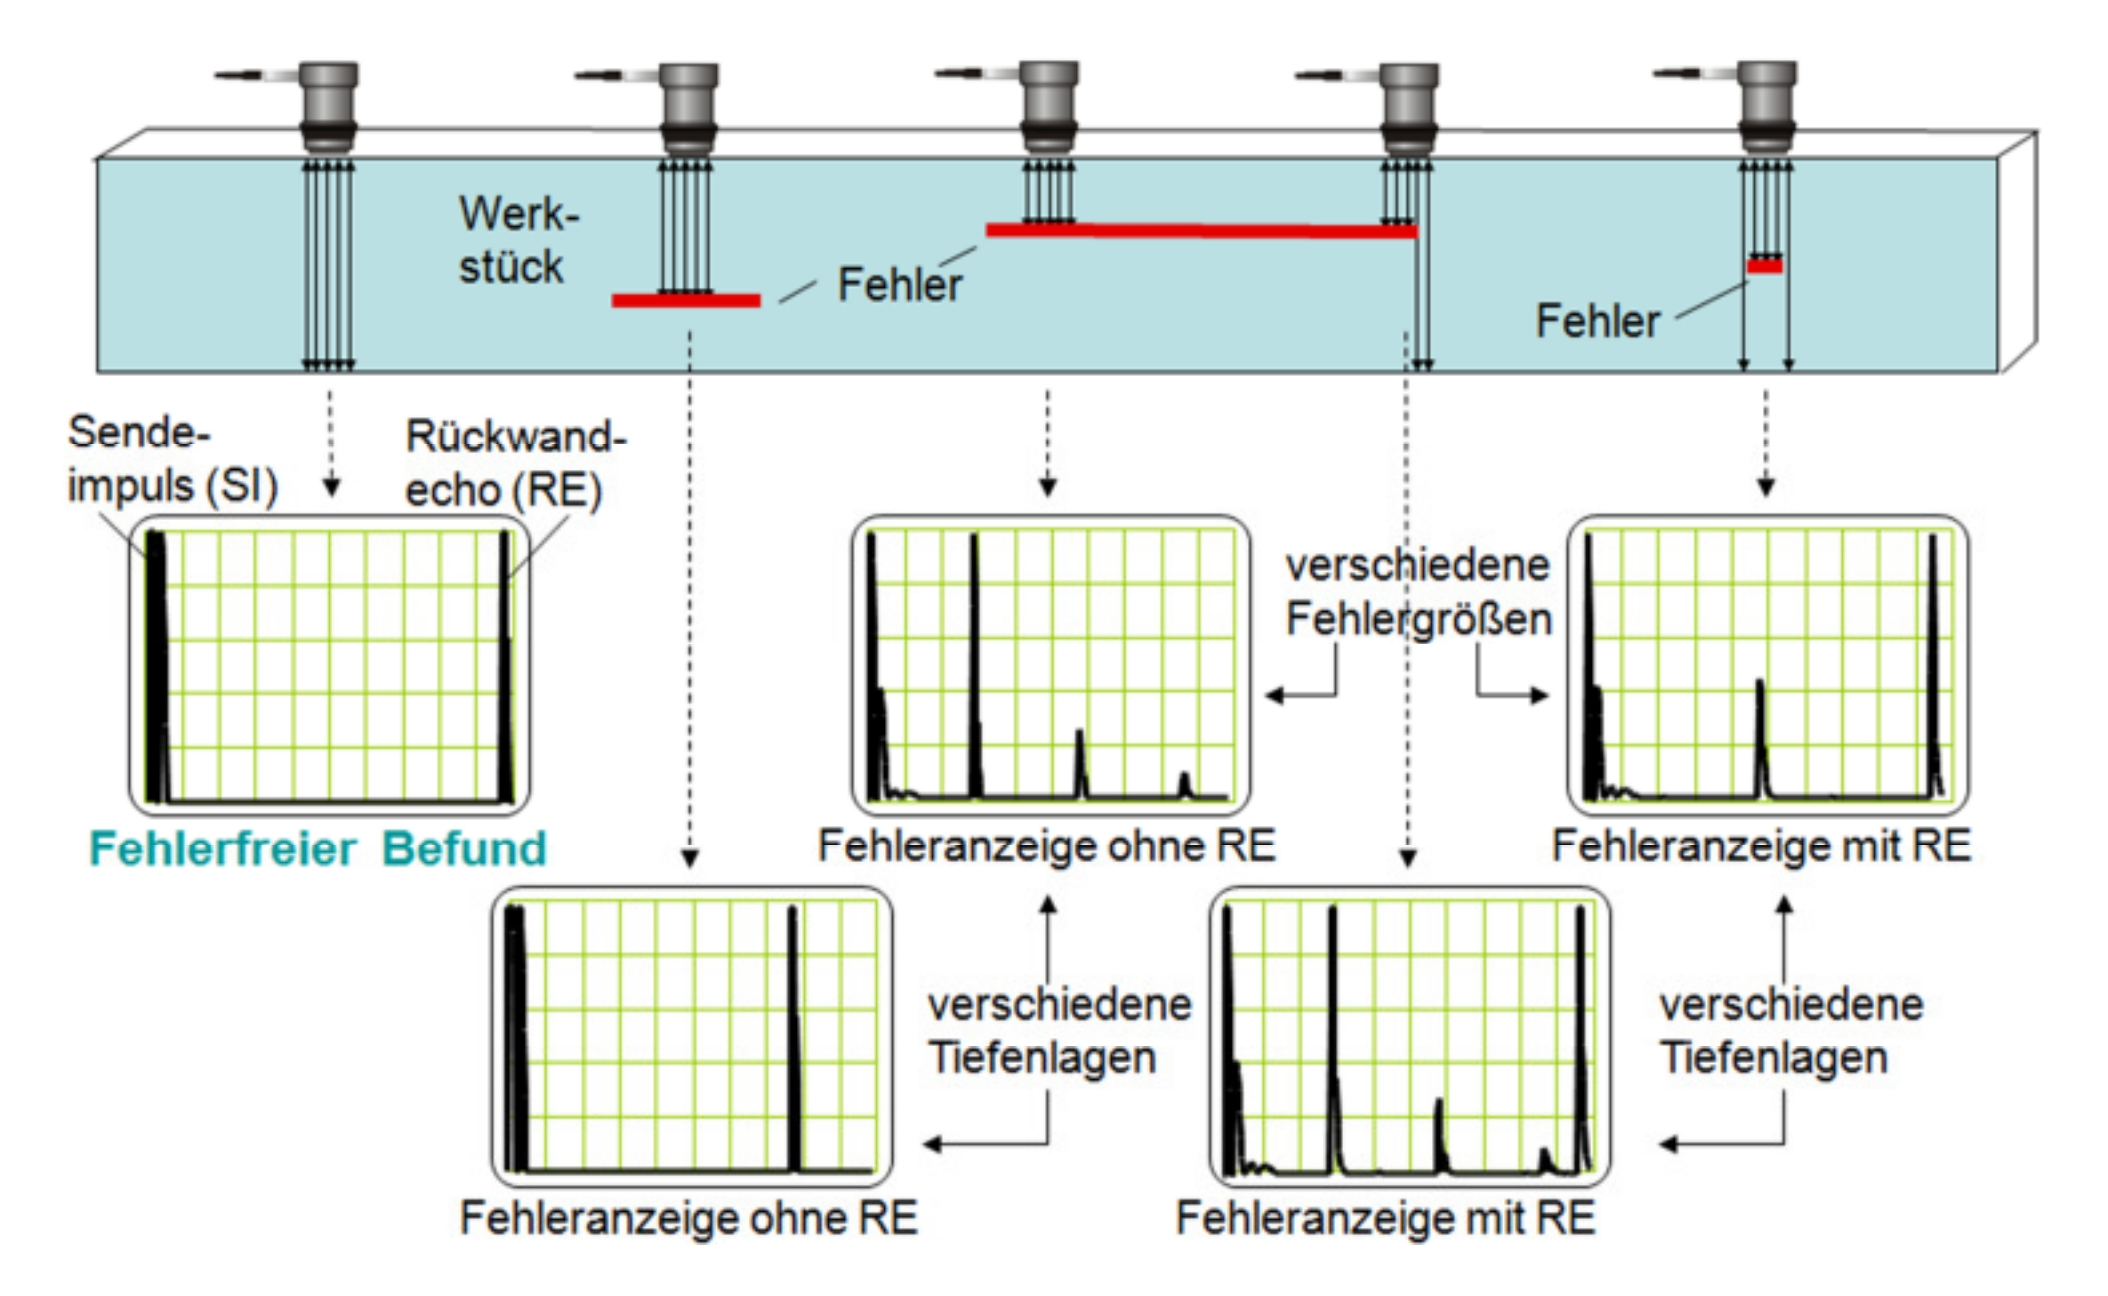
\includegraphics[width=0.72\textwidth]{pictures/Oszillogramme.jpg}
\caption{Oszillogramme (beispielhaft, Nummer eins bis fünf von links nach rechts)\footnotemark }
%TODO Quelle funktionierend angeben
\end{center}\end{figure}\footcitetext{img:oszillogramm} \\
Je höher dabei eine Spitze (auch Peak) ist, desto stärker war das zugehörige Echo. 
Hierbei wird ausgenutzt, dass beim Übergang der Ultraschallwellen von einem Material zum anderen ein bestimmter Anteil reflektiert wird, während ein anderer Anteil (unter einem anderen Winkel) sich weiter durch den Körper bewegt. 
Trifft eine Schallwelle, die sich in einem festen Körper bewegt, auf Luft, so wird sie beinahe vollständig zurückgeworfen, weshalb etwaige passierende Schallwellen gering genug sind, um vernachlässigt werden zu können. 
So erscheint das erste Echo schon direkt zu Beginn der Messung, wie im ersten Oszillogramm zu sehen: Es entsteht, wenn die ausgesandten Wellen in den Probekörper eintreten. Denn zwischen Prüfkopf und Prüfkörper befindet sich immer eine (meist sehr dünne) Luftschicht; daher wird der Schall schon einmal reflektiert, bevor der relevante Teil des Verfahrens beginnt. 
Um dies in der Praxis zu minimieren, wird eine Kopplungsflüssigkeit verwendet, welche den Schall mit möglichst wenig Reflexionen zwischen Werkstück und Prüfkopf transportiert. 
Das zweite Echo stellt in diesem Fall das sogenannte Rückwandecho dar, bei welchem die Wellen von der dem Prüfkopf gegenüberliegenden Seite zurückgeworfen werden. 
Mithilfe dessen kann auch Tiefe des Prüfkörpers ermittelt werden.
Da der Schall stets eine materialspezifische Geschwindigkeit $c_\mathrm{Material}$  \footcite{schallgeschwindigkeiten}
besitzt, gilt für die Stärke des Körpers: $d = \dfrac{c_{\mathrm{Material}} \cdot t}{2}$. 
Dies ist vor allem hilfreich, wenn Probeköper nur von einer Seite erreichbar sind und ihre Dimensionen daher nicht mit herkömmlichen Werkzeugen bestimmt werden können.\\
Für die zerstörungsfreie Prüfung ist diese Möglichkeit jedoch eher von geringerer Bedeutung. 
Der eigentliche Nutzen von Ultraschall lässt sich besser an den anderen Oszillogrammen erklären. 
Befinden sich Fehler im Werkstück, sind das meist Lufteinschlüsse in Form von Rissen oder Löchern. 
Da sich somit auch dort ein Materialübergang befindet, werden Schallwellen an Fehlstellen ebenfalls reflektiert. 
Analog zur Bestimmung der Maße des Körpers können auch die ungefähren Positionen der Fehler ermittelt werden. 
Der große Vorteil dieses Verfahrens ist, dass es nahezu unbegrenzt einsetzbar ist, da sich Sender und Empfänger in einem Gerät befinden und so auch bei komplexen Geometrien, welche nur eingeschränkt zugänglich sind, genutzt werden können. 
Problematisch ist hingegen die Auswertung der entstehenden Oszillogramme. 
Zum Beispiel Oszillogramm Nummer vier: Einerseits gibt es das normale Rückwandecho, also befindet sich der Prüfkopf teilweise über einem Streifen ohne Fehler; zusätzlich existieren jedoch noch weitere Echos, die auf Fehlstellen hinweisen. 
Eine mögliche Deutung wäre, dass es mehrere verschieden große Lufteinschlüsse in unterschiedlichen Tiefen gibt, welche die Echos verursachen. 
Diese Interpretation wäre allerdings falsch, denn wie man sehen kann, gibt es nur einen Fehler, von dem das Echo immer wieder reflektiert wird. 
An dieser Stelle muss man anmerken, dass in diesem Fall kein gutes Kopplungsmittel verwendet wurde, da sonst das Echo sehr viel schneller abschwächen würde. 
Der Grund dafür, dass es dennoch schwächer wird, ist einerseits der Fakt, dass die Wellen teilweise die Fehlstelle passieren und somit ein wenig ihrer Stärke verlieren, andererseits aber auch die Streuung der Schallwellen im Körper, sodass das Signal stetig schwächer wird.\\
Im Detail kann die Verfahrensweise der zerstörungsfreien Materialprüfung mit Ultraschall nachgelesen werden in Quelle 
\footcite{karldeutsch}. 

\subsection{Abgrenzung von anderen Testverfahren}

Obwohl die zerstörungsfreie Prüfung mittels Ultraschall in der heutigen Wirtschaft unverzichtbar ist, kann mithilfe der Ultraschallmesstechnik nicht jeder Materialtest durchgeführt werden, da auch diese durch die Grundlagen der Physik eingeschränkt wird.
Um diese Grenzen zu überwinden, wird auf andere Materialeigenschaften zurückgegriffen.
Dabei handelt es sich um optische, thermische, elektrische, magnetische und atomare Eigenschaften des Prüflings. 
Jede der Methoden bietet dabei eigene Vor- und Nachteile und ist damit für spezielle Prüfvorgänge geeignet. \\ 
Grundsätzlich unterscheiden sich diese Verfahren in ihren Anforderungen an technische Geräte und dem benötigten Fachwissen, diese zu bedienen und den Prüfvorgang ordnungsgemäß durchzuführen. 
Diese versucht man natürlich möglichst gering zu halten, um viele Bauteile effizient prüfen zu können.
Daher sind die am häufigsten verwendeten Verfahren die Sichtprüfung und die Farbeindringprüfung. 
Bei diesen wird entweder mit bloßem Auge oder mithilfe von farbigen Flüssigkeiten die Oberfläche von Prüflingen auf Fehler begutachtet. 
Dies kann schnell, einfach und ohne technischen Aufwand durchgeführt werden.
Doch durch den Ablauf beim Prüfen werden auch die Nachteile dieser Verfahren klar, denn unter Verwendung des Auges oder von Kameras kann nur die Oberfläche von Prüfkörpern beurteilt werden. \\
Dies ist für einige Teile ausreichend, doch besonders stark beanspruchte oder sicherheitsrelevante Teile dürfen auf keinen Fall versagen. 
Oft reicht hier schon ein kleiner Riss im Inneren, um genau dieses Versagen herbeizuführen. 
Daraus ergibt sich die Notwendigkeit, in diesen Fällen den Prüfkörper auch auf innere Beschädigungen zu untersuchen.
Dazu stehen ebenfalls mehrere Methoden zur Verfügung.
Abhängig von Größe und Material des Prüflings sind manche Testverfahren besser geeignet als andere. 
So basieren z.B. manche Verfahren auf der elektrischen Leitfähigkeit des Prüfkörpers und sind daher auf bestimmte Materialien beschränkt.
Andere hingegen erfordern geschlossene Sicherheitsräume, wie z.B. die Röntgenprüfung, und können daher schlecht zur Prüfung von bereits verbauten Teilen verwendet werden.\\
Allerdings kann auch durch die verwendete Methode selbst eine Einschränkung erfolgen. So ist z.B. beim Prüfen mit Ultraschall die Materialdicke -- abhängig vom verwendeten Prüfgerät -- auf fünf bis acht Meter beschränkt, da sonst Ungenauigkeiten entstehen könnten. \footcite{ultraschall} \\ 
Das Ultraschallverfahren, dessen Simulation Thema dieser Arbeit ist, bietet insgesamt eine gute Kombination praxisrelevanter Eigenschaften.
So können bei relativ geringem technischen Aufwand und unter Verwendung mobiler Prüfgeräte kleine bis mittelgroße Prüfkörper relativ genau auf innere Fehler untersucht werden.

\section{Berechnung der Strahlenverläufe}

\subsection{Grundbegriffe und Notation der Vektorrechnung}
Im Folgenden sollen die zur Berechnung verwendeten Formeln erklärt und hergeleitet werden. 
Dazu ist es nötig, einige Bezeichnungen einzuführen: Wie allgemein üblich, werden wir einen Vektor, welcher sich als \glqq Schritt\grqq{} im Raum versinnbildlichen lässt, durch einen Pfeil darüber kennzeichnen, zum Beispiel $\vec{v}$. 
Weiterhin soll der Ortsvektor eines Punktes (also der Vektor vom Koordinatenursprung zu dem Punkt) mit dem zum Großbuchstaben des Punktes gehörenden Kleinbuchstaben bezeichnet werden. Der Punkt $O(4|2)$ hat also den Ortsvektor $\vec{o} = \vect{4}{2}$. 
Zudem verweist ein tiefgestelltes $x$ auf die Komponente eines Vektors beziehungsweise eines Punktes in x-Richtung und ein $y$ auf die y-Komponente. 
Auf das soeben genannte Beispiel bezogen gilt $O_x = \vec{o}_x = 4$ und $O_y = \vec{o}_y = 2$.

\subsection{Erklärung und Begründung der vorgenommenen Vereinfachungen}

\subsubsection{Die Notwendigkeit von Vereinfachungen} %TODO Wir verwenden "Körper" statt Formen/ Flächen
Da das Programm die Berechnungen in akzeptabler Zeit durchführen können soll, dürfen die verwendeten Formeln nicht zu umfangreich sein. 
Außerdem ist eine exakte Simulation nicht nötig, da der Nutzer den jeweiligen Prüfkörper ohnehin nur annähernd digitalisieren kann, weshalb berechnete Ergebnisse, unabhängig von der Art der Berechnung, meist nicht genau mit den realen Messwerten übereinstimmen werden. 
Daher ist es legitim, einige mathematische und physikalische Vereinfachungen vorzunehmen, um die \hyperref[sec:herleitung]{Herleitung der Formeln} möglichst unkompliziert zu gestalten. 
Welche Näherungen mit welcher Intention vorgenommen wurden, soll in diesem Kapitel näher beleuchtet werden.

\subsubsection{Betrachtung der Ultraschallwellen als Strahlenbündel}
Genau wie jede andere Art des Schalls ist Ultraschall eine mechanische Welle und breitet sich daher dem Huygens'schen Prinzip folgend allseitig aus. 
Jedoch ist die Amplitude und somit auch die Intensität der Welle in einer Richtung wesentlicher stärker.
Der Aufbau des Senders ermöglicht es, den Schall zu fokussieren, um spezifische Bereiche des Körpers prüfen zu können.
Die Ausbreitung einer Welle, inklusive der Reflexion beim Übergang von einem Medium in ein anderes, zu berechnen ist sehr kompliziert, besonders da sie schlecht als Datenstruktur dargestellt werden kann.\\
An dieser Stelle kommt die Vektorrechnung ins Spiel: Indem angenommen wird, dass sich der Schall in nur eine Richtung ausbreitet, kann man ihn als Strahl betrachten. 
Mathematisch gesehen besteht er also aus einem Ortsvektor zum Startpunkt und einem Richtungsvektor. 
Die vektorielle Darstellung eines Strahls $\vec{v}$, der in einem zweidimensionalen kartesischen Koordinatensystem mit dem Koordinatenursprung $O(0|0)$ am Punkt $P(0|3)$ beginnt und von dort aus in Richtung des Punktes $Q(1|4)$ verläuft, lautet also $\vec{v} = \overrightarrow{OP} + \lambda \cdot \overrightarrow{PQ} = \vect{0}{3} + \lambda \cdot \vect{1}{1}$, wobei $\lambda\in\mathbb{R}$ und $\lambda\geq0$ gilt. 
Dieses Vorgehen bringt große Vorteile mit sich. Beispielsweise ist es mithilfe dessen sehr einfach, Schnittpunkte und Reflexionsvektoren auszurechnen, wie in Kapitel \ref{sec:herleitung} beschrieben.\\
Natürlich muss die dadurch entstehende Vernachlässigung der allseitigen Ausbreitung kompensiert werden. 
Aus diesem Grund werden nicht nur einer, sondern mehrere solcher Strahlen von der Quelle ausgesandt. 
Somit entfällt einerseits die Problematik der Reflexion einer gesamten Wellenfront an einem Objekt, welche sehr umständlich ist, andererseits bleibt die Genauigkeit nahezu erhalten. 
Wird in einem realen Prüfkörper ein großer Teil des Schalls zurück zum Sender reflektiert, passiert dasselbe auch in der Simulation. 
Der Unterschied besteht allein darin, dass in einer realen Messung die registrierte Schallintensität analog ist, da sie auch von Feinheiten im Prüfling beeinflusst wird, während das Programm eine digitale Intensität feststellt, denn diese ist abhängig von der Anzahl der reflektierten Strahlen, welche selbstverständlich eine natürliche Zahl sein muss.\\
Aufgrund dessen entsteht eine geringe Abweichung der Berechnung von der Messung, jedoch kann diese Abweichung minimiert werden, indem möglichst viele Strahlen ausgesandt werden, was die \glqq Lücken\grqq{} zwischen den digitalen Zahlen verkleinert. 
Dies impliziert zwar einen höheren Rechenaufwand, jedoch kann die Strahlenanzahl für die meisten Simulationsparameter (wie zum Beispiel die Form des Prüfkörpers und Anzahl der Reflexionen) so gewählt werden, dass sowohl die Qualität des Ergebnisses als auch die zur Berechnung benötigte Zeit akzeptabel sind.

\subsubsection{Berechnung der Intensität eines einzelnen Strahls}
Neben der Anzahl der zurückgekommenen Strahlen gibt es für den Sender einen weiteren Parameter dafür, wie stark der Peak des Oszillogramms an einem bestimmten Zeitpunkt sein muss. 
Aus der Länge des Weges jedes Strahls wird berechnet, wie groß seine Intensität bei der Rückkehr ist. 
Näher beleuchtet wird dies in Kapitel \ref{sec:sim}.\\
Durch die auftretende Reibung zwischen den schwingenden Teilchen kommt es dazu, dass die Ultraschallwellen abhängig von der zurückgelegten Strecke an Energie verlieren.
Für unsere Simulation sind wir dabei von einer exponentiellen Funktion $I = \frac{I_0}{1.05^{\tfrac{s}{c}}}$ zur Berechnung der Intensität $I$, mit $I_0$ als Ausgangsintensität, $s$ als zurückgelegter Weg und $c$ als materialspezifische Schallgeschwindigkeit, ausgegangen.

\subsubsection{Vernachlässigung der Materialübergänge und Annahme der Totalreflexion}
In unserer Arbeit gehen wir davon aus, dass der gesamte Prüfkörper aus einem einzigen Material besteht. 
Dies bringt zum Einen den Vorteil, dass die genannte Formel zur Berechnung der Intensität eines Strahls angewendet werden kann, da die Schallgeschwindigkeit so konstant ist. 
Existierten mehrere Materialien, so würde sie sich während des Durchlaufs durch den Prüfkörper ändern und würde so die Berechnung erschweren. 
Weiterhin finden an Materialübergängen wellenphysikalische Vorgänge wie Brechung und Reflexion statt, welche den Verlauf der Strahlen direkt beeinflussen. 
Das Problem ist vor allem, dass sich dabei die Energie des ursprünglichen Strahls in den gebrochenen und den reflektierten Anteil aufspaltet, wodurch sehr schnell sehr viele separate Strahlen aus einem einzigen Ursprungsstrahl entstehen, welche jeweils einzeln berechnet werden müssen und somit in der Summe einen großen Rechenaufwand darstellen. 
All dies ist zwar prinzipiell leicht zu berechnen, wenn klare Grenzen zwischen den verschiedenen Stoffen bestehen, jedoch nicht, wenn diese eher \glqq fließend\grqq{} ineinander übergehen.\\
Daraus folgt weiterhin, dass es sich erübrigt, eine allgemeine Formel zur Berechnung des reflektierten Schalls zu verwenden. 
Es wird davon ausgegangen, dass der einzige Materialübergang zwischen dem Prüfkörper und seiner Umgebung, also Vakuum, besteht. 
Näherungsweise ist dies gleichzusetzen mit einem Übergang zwischen dem Prüfkörper und Luft. 
Da sich die Schallgeschwindigkeit in Luft sehr stark von derjenigen in festen Stoffen unterscheidet, wird beinahe der gesamte Anteil des Strahls reflektiert, was aus Gründen der Berechenbarkeit als tatsächliche Totalreflexion angesehen wird. 
Somit kann die Reflexion als rein mathematisches Problem der Vektorrechnung ohne physikalische Beschränkungen betrachtet werden.

\subsection{Herleitung der Reflexiongleichungen}\label{sec:herleitung}

\subsubsection{Reflexion an einer Geraden}
Durch die Verwendung der Vektorrechnung lässt sich für unsere Arbeit die Reflexion eines Strahls an einer beliebigen regelmäßigen Geometrie auf die Reflexion eines Strahls an einer Geraden zurückführen. 
Diese ist damit ein essenzieller Prozess, der häufig durchgeführt werden muss.\\
\begin{wrapfigure}{rH}{10.5cm}
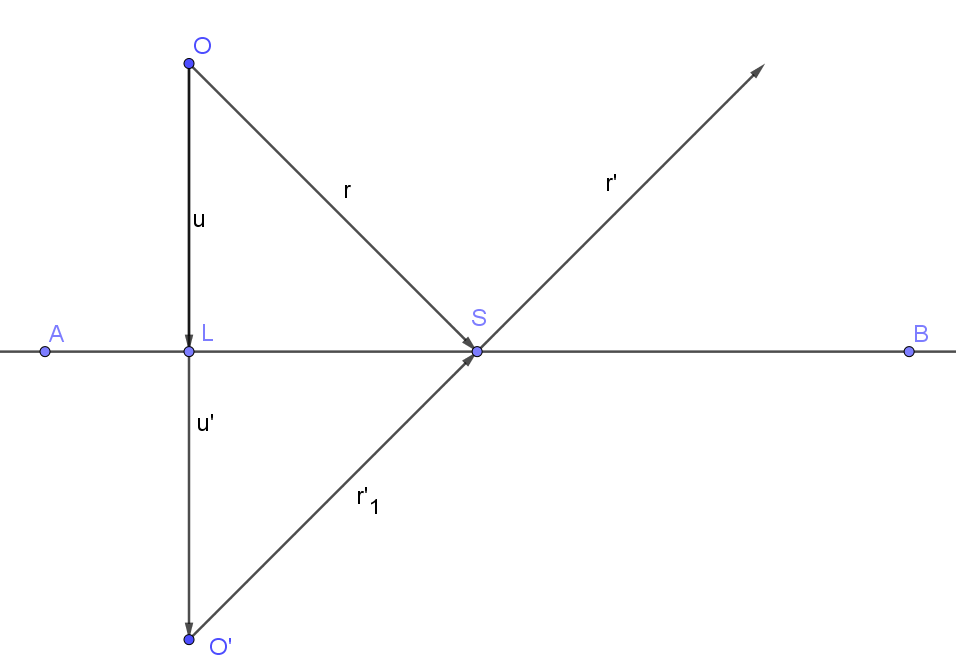
\includegraphics[scale=0.4]{pictures/LineRef.png}
\caption{Reflexion an einer Geraden}
\end{wrapfigure}
Um die Berechnung des reflektierten Strahls durchzuführen, müssen sowohl zwei Punkte der Geraden, $A$ und $B$, gegeben sein, als auch der Ausgangspunkt $O$ und der Richtungsvektor $\vec{r}$ des Ausgangsstrahls. 
Mittels des Vektors $\vec{u} = 2\cdot\overrightarrow{OL}$ zwischen $O$ und dem Lotfußpunkt $L$ von $O$ auf $\overline{AB}$ ergibt sich auch $\vec{o'} = \vec{o} + 2\cdot\vec{u}$ und damit der Spiegelpunkt $O'$ von $O$ an $AB$.
Weiterhin ist der Schnittpunkt $S$ des Strahls von $O$ in Richtung $\vec{r}$ mit der Geraden $AB$ durch die Formel
\begin{center}
$\vec{s} = \vec{o} - \dfrac{O_x \cdot \vec{r}_y - O_y \cdot \vec{r}_x - A_x \cdot \vec{r}_y - A_y \cdot \vec{r}_x}{A_x \cdot \vec{r}_y - A_y \cdot \vec{r}_x - B_x \cdot \vec{r}_y + B_y \cdot \vec{r}_x} \cdot \vec{r}$
\end{center}
bestimmt. 
Daraus ergibt sich folgend der Vektor
\begin{center}
$\vec{r'} = \vec{r'_1} = \overrightarrow{O'S}$
\end{center}
und damit auch der neue Strahl von $S$ in Richtung $r'$.

\subsubsection{Reflexion an weiteren regelmäßigen Geometrien} \label{sec:weitereGeometrien}
Neben der Reflexion der Strahlen an einer einfachen Geraden haben wir uns auch entschieden, dies für Kreise, Kreisbögen und Ovale herzuleiten und zu implementieren. 
Grundsätzlich erfolgt dabei auch die Reflexion an einer Geraden, doch diese muss in Abhängigkeit von der Form erst einmal bestimmt werden. 
Für folgende Herleitungen wird erneut von einem Strahl, der in $O$ beginnt und sich in Richtung $\vec{r}$ ausbreitet, ausgegangen.
\begin{wrapfigure}[18]{rH}{8.5cm}
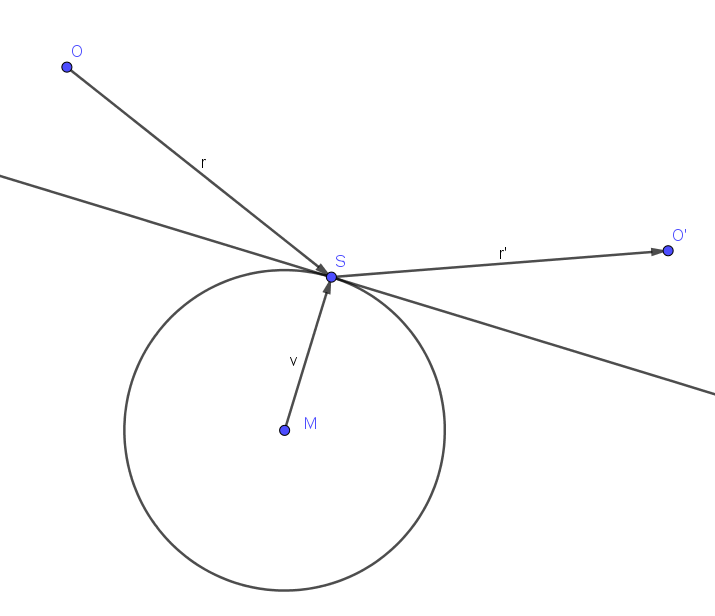
\includegraphics[scale=0.5]{pictures/CircleRef.png}
\caption{Reflexion an einem Kreis}
\end{wrapfigure}
Die zur Berechnung notwendige vektorielle Darstellung des Kreises $K(M, r)$ erfolgt in der Form $K: \vec{x} = \vec{m} + \vec{v}$ mit $|\vec{v}| = r$.
Mithilfe dessen wird zunächst der Punkt bestimmt, in welchem der Strahl den Kreis schneidet, indem das folgende Gleichungssystem nach den drei unbekannten Variablen $\lambda$, $\vec{v}_x$, $\vec{v}_y$ gelöst wird:
\begin{equation*}
\begin{split}
\vec{k}_x + \vec{v}_x & = O_x + \lambda\cdot\vec{r}_x\\
\vec{k}_y + \vec{v}_y & = O_y + \lambda\cdot\vec{r}_y\\
r^2 & = \vec{v}_x^{~2} + \vec{v}_y^{~2} 
\end{split}
\end{equation*}
Das so ermittelte $\lambda$ wird in die Formel $\vec{s} = \vec{o} + \lambda \cdot \vec{r}$  eingesetzt, um den Schnittpunkt $S$ zu berechnen. 
Durch den Vektor $\vec{n} = \vec{MS}$ zwischen Kreismittelpunkt und Schnittpunkt lässt sich leicht die Tangente in $S$ mit $T: ~\vec{x} = \vec{s} + \lambda \cdot \begin{pmatrix} -n_y \\ n_x \end{pmatrix}$ ermitteln.
Somit kann die Reflexion am Kreis auf eine Reflexion an einer Geraden zurückgeführt werden.\\
Die Reflexion an Kreisbögen funktioniert analog, aus einem Kreisbogen wird der entsprechende vollständige Kreis gebildet, an welchem wie beschrieben reflektiert wird. 
Jedoch muss zusätzlich noch überprüft werden, ob der Schnittpunkt mit dem \glqq Hilfskreis\grqq{} auch auf dem Teil des Kreises liegt, den dieser mit dem Kreisbogen teilt. 
Dies geschieht derart, dass festgestellt wird, ob der Winkel des Kreissektors vom Startpunkt des Kreisbogens bis zum Schnittpunkt kleiner ist als der Winkel des Kreissektors, welchem der Kreisbogen insgesamt entspricht. 
Dazu wird eine Formel zur Berechnung des Winkels in mathematisch positiver Richtung von einem Vektor $v$ zu einem anderen Vektor $w$ $\sphericalangle(\vec{v}, \vec{w}) = -\atantwo(\vec{v}_x\cdot\vec{w}_y-\vec{v}_y\cdot\vec{w}_x,~\vec{v}_x\cdot\vec{w}_x+\vec{v}_y\cdot\vec{w}_y)$  verwendet.
\newpage
\begin{wrapfigure}[14]{rH}{9cm}
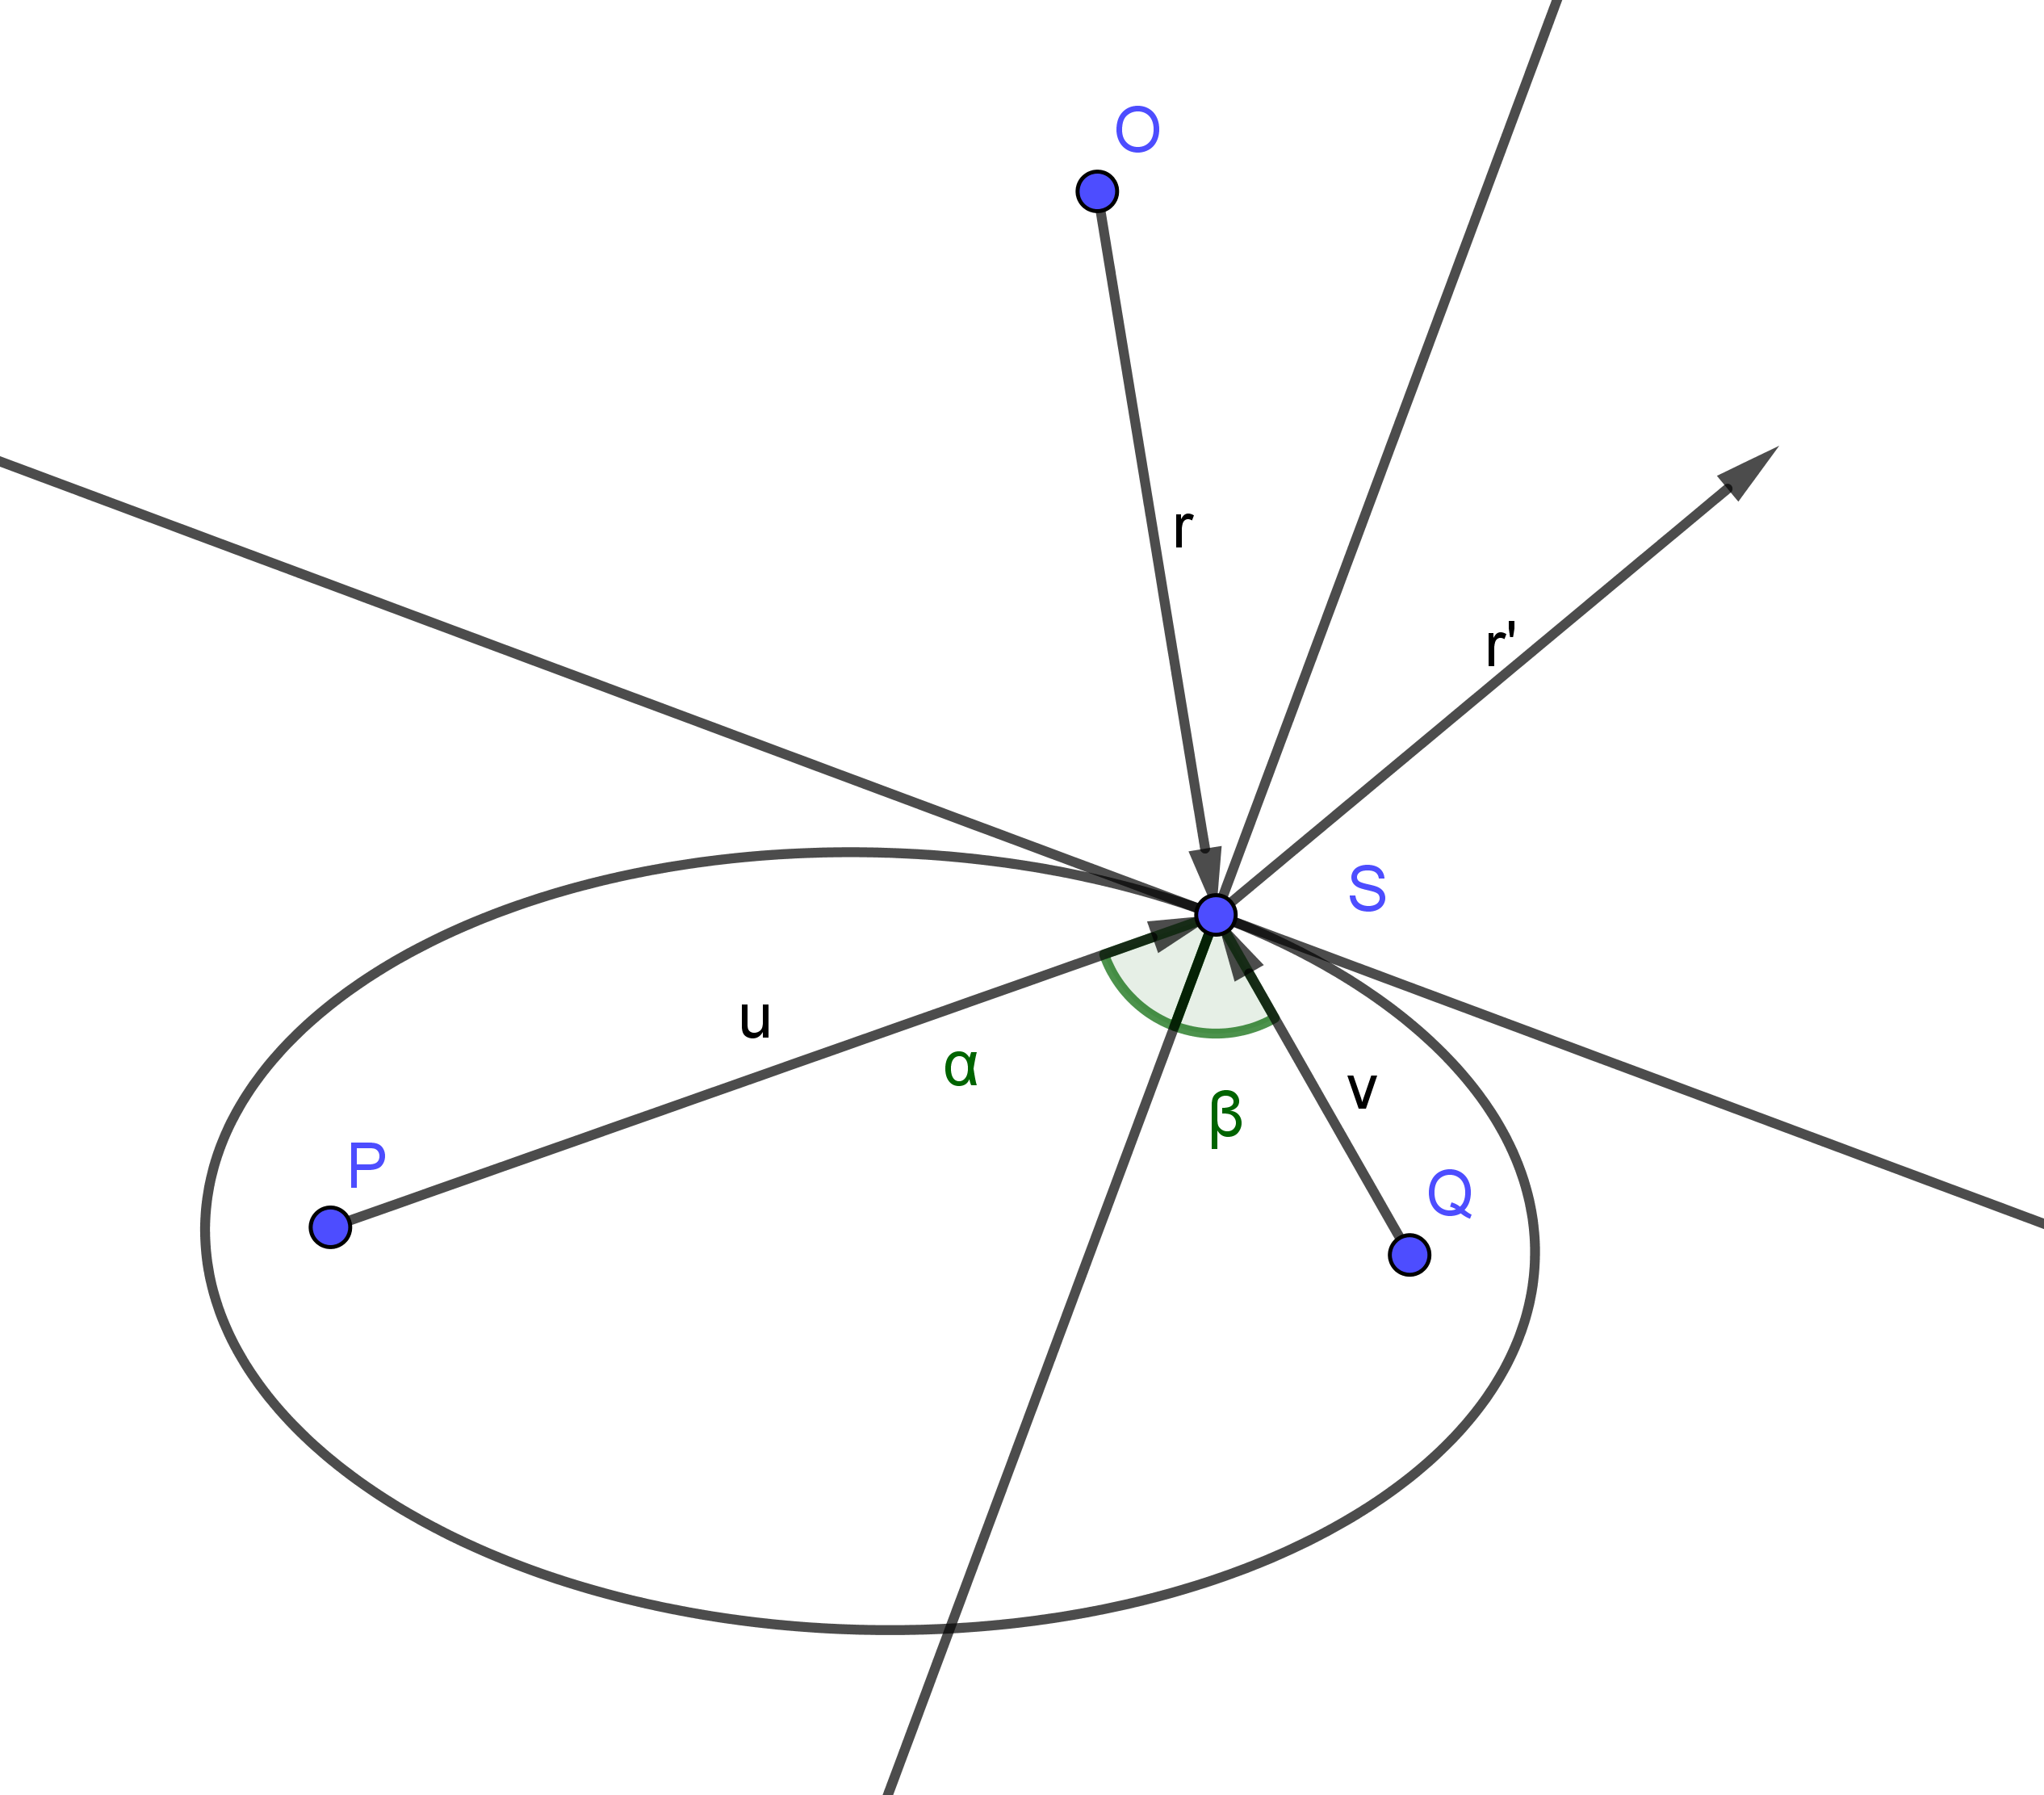
\includegraphics[scale=0.7]{pictures/OvalRef.png}
\caption{Reflexion an einer Ellipse}
\label{fig:Ellipse}
\end{wrapfigure}
Als letzte Form haben wir die Ellipse $E(P, Q, e)$ implementiert.
Wie beim Kreis ist es nötig, eine vektorielle Darstellung zu finden. 
Aufgrund der Definition einer Ellipse lautet diese $E: \vec{x} = \vec{p} + \vec{u} = \vec{q} + \vec{v}$ mit $ e = |\vec{u}| + |\vec{v}|$.
Zur Bestimmung des Schnittpunkts $S$ wird nun folgendes Gleichungssystem nach $\lambda$ gelöst:
\begin{equation*}
\begin{split}
\vec{o} + \lambda \cdot \vec{r} &= \vec{p} + \vec{u} \\
\vec{o} + \lambda \cdot \vec{r} &= \vec{q} + \vec{v} \\
\vec{p} + \vec{u} &= \vec{q} + \vec{v} \\
|\vec{u}| + |\vec{v}| &= e
\end{split}
\end{equation*}
Daraus ergibt sich folgend der Punkt $S$ mit $\vec{s} = \vec{o} + \lambda \cdot \vec{r}$.\\
Um nun am Schnittpunkt eine Reflexion durchzuführen, ist es erneut notwendig, eine Tangente an das Oval anzulegen. 
Dies erfolgt unter Ausnutzung der Brennpunkteigenschaft. \footcite{beweis-ellipse}
Nach dem Satz vom Flüstergewölbe gilt für Brennstrahlen in Ellipsen, im Beispiel aus Abbildung \ref{fig:Ellipse} $\overline{PS}$ und $\overline{QS}$, dass die Winkelhalbierende der beiden Strahlen die Normale zur Tangente im Punkt der Ellipsenperipherie, hier $S$, ist.
Unter Ausnutzung dieser Eigenschaft lässt sich für Ellipsen eine Gleichung zur Herleitung einer Tangente $T(S)$ aufstellen.\\
Um die Winkelhalbierende $\vec{n}$ zwischen den Brennstrahlen zu erhalten, werden diese normiert und aufaddiert.
\begin{equation*}
\begin{split}
\vec{u'} & = \dfrac{\vec{u}}{|\vec{u}|} \\
\vec{v'}  &= \dfrac{\vec{v}}{|\vec{v}|} \\ \\
\vec{n} & = \vec{u'} + \vec{v'} \\ 
\end{split}
\end{equation*}
Schließlich ist die Tangente lediglich der Vektor senkrecht auf der Normalen, der durch den Schnittpunkt $S$ verläuft.
\begin{equation*}
\begin{split}
T: \vec{x} & = \vec{s} + \lambda \cdot \begin{pmatrix} -n_y \\ n_x \end{pmatrix}
\end{split}
\end{equation*}
Damit lässt sich auch die Reflexion an einer Ellipse auf die an einer Geraden zurückführen.\\
Aus Platzgründen mussten wir die ausführliche Herleitung einiger Formeln hier auslassen, diese sind im Kapitel \ref{sec:AnhangHerlFormel} zu finden.

\newpage
\section{Erstellen eines Programms zur Prüfungssimulation }\label{sec:sim}

\subsection{Anforderungen an das Programm}

Das im Rahmen der Arbeit entstandene Programm soll in erster Linie für zwei Zwecke eingesetzt werden können: Das Finden eines Prüfansatzes für komplexe Prüfkörper und die Validierung uneindeutiger Hypothesen basierend auf Messungen an solchen Prüfkörpern.
Um dies zu ermöglichen, muss das Programm beliebig komplexe zweidimensionale Geometrien umsetzen können. 
Dies geschieht im sogenannten Körpereditor, in dem der Nutzer aus einer Reihe von Figuren wie Ovalen, Kreisen und Polygonen sowohl die geplante Form des Prüflings - im Programm \textit{Outline} - als auch eventuelle Fehler - im Programm \textit{Defects} - zusammenfügen kann. \\
Daraus ergibt sich eine naheliegende Begrenzung des Programms. 
In der Praxis hat ein Prüfer Kenntnis der Outline und der Messergebnisse und muss daraus auf die Position und Art der Defekte schließen. 
Das Simulationsprogramm hingegen schließt aus der Kenntnis der Outline und Defekte die Form der Messergebnisse, d.h. es simuliert die Messung. 
Dies steht in unmittelbarem Zusammenhang mit den beabsichtigten Anwendungsszenarien.
Besteht nur eine ungefähre Vermutung über die Position möglicher Fehler, etwa in einer bestimmten, schwierig zu erreichenden Ecke eines konkaven Prüfkörpers, so kann der Nutzer die bekannte Outline des Körpers nachbauen und mit verschiedenen Senderpositionen und Einfallswinkeln experimentieren, um einen guten Prüfansatz zu finden. 
Das dabei entstehende Oszillogramm dient dann als Vorlage für eine fehlerfreie Messung. \\
Als zweites Anwendungsfeld ergibt sich die Validierung von Hypothesen. 
Ultraschall-Messungen geben oft keine eindeutige Auskunft über die Form und Position der Fehler. 
Diese Schlussfolgerungen zu ziehen, ist Aufgabe eines Prüfers. 
Es kann aber gerade bei komplexen Geometrien hilfreich sein, zu überprüfen, ob die vermutete Position des Fehlers tatsächlich zu den vorliegenden Messergebnissen führen würde. \\
Neben dem Prüfling kann der Nutzer auch den Messaufbau verändern, indem er Position und Einfallswinkel des Senders verändert. 
Auch im Simulationsfenster können Änderungen an der Position und Form des Prüfkörpers und der Defekte vorgenommen werden, was eine geringfügige Veränderung der Situation ermöglicht, ohne den Körpereditor zu verwenden.
Startet der Nutzer die Simulation, erhält er zum einen eine Darstellung des Strahlenverlaufs im Prüfkörper und zum anderen eine grobe Form des entstehenden Oszillogramms, die im Wesentlichen aus den Peaks der Messung besteht. \\
Das Programm ist als eine Java-Anwendung umgesetzt, da die Programmiersprache aus dem Unterricht bekannt ist und sich mittels des GUI-Toolkits Swing für die Darstellung einfach zu bedienender Benutzeroberflächen eignet.
Weiterhin wird für die Berechnungen eine Python-Bibliothek mit gleichem Funktionsumfang, aber ohne die dazugehörige Benutzeroberfläche entwickelt.

\subsection{Simulation und Darstellung der Ultraschallprüfung}

\subsubsection{Raytracer und und die trace-Funktion}
Die im vorangegangenen Kapitel hergeleiteten Formeln sind in der Klasse \textsc{Raytracer} implementiert. 
Daher existiert für jede geometrische Form eine Methode zum Berechnen des Schnittpunktes mit dem Strahl und eine zur Berechnung des reflektierten Vektors und somit des neuen Strahls. 
Weiterhin gibt es spezielle Prozeduren, um das Problem der Reflexion in einer Ecke zu behandeln.\\
Das Kernstück der Klasse ist jedoch die \texttt{trace}-Funktion, welche dazu dient, den gesamten Verlauf eines Strahls im Prüfkörper zu ermitteln. 
Dazu wird mithilfe der Schnittpunkt-Funktionen der Schnittpunkt mit jedem Objekt in dem Körper ermittelt, sofern existent. 
Anschließend wird die Reflexionsmethode für dasjenige Objekt aufgerufen, welches tatsächlich vom Strahl getroffen wird, also dessen Schnittpunkt mit dem Strahl am nächsten an dem Ausgangspunkt des Strahls liegt. 
Sind mehrere Objekte gleich weit entfernt, wird die Funktion zur Reflexion an Ecken aufgerufen, sodass in jedem Fall ein eindeutiger neuer Strahl entsteht.\\
Bei jeder einzelnen Reflexion wird der vorherige Strahl in einer Liste gespeichert, sodass am Ende sämtliche Strahlen mit Anfangspunkt und Richtungsvektor geordnet in dieser Liste stehen. 
Mithilfe dessen ist der Verlauf des Strahls durch den Prüfkörper eindeutig nachvollziehbar, indem die Reflexionspunkte in der gegebenen Reihenfolge betrachtet werden.

\subsubsection{Scansimulation mit Einfach- und Mehrfachstrahl}
Die Simulation der Scanverfahren und die finale Berechnung und Auswertung der Reflexionen wird in der Klasse \textsc{Scan} umgesetzt.
Basierend auf den von \textsc{Raytracer} ermittelten Punkten, an welchen die Strahlen reflektiert werden, errechnet man, welche Zeit zwischen den einzelnen Reflexionen vergeht.
Weiterhin wird für jeden Auftreffpunkt geprüft, ob dieser im Messbereich des Senders liegt. 
Ist dies der Fall, so wird in Abhängigkeit von der bereits verstrichenen Zeit die Intensität ermittelt. 
Insgesamt geht man hierbei von einer über die Zeit exponentiell fallenden Intensität aus.\\
Ähnlich verhält es sich auch bei der Simulation mit mehreren Strahlen. 
Hierfür werden die Strahlen gleichmäßig über den gegebenen Streuwinkel verteilt und für jeden Strahl die zuvor erklärte Prozedur durchgeführt. 
Schließlich werden alle ermittelten Wertepaare aus Zeit und Auftreffintensität zusammengefasst.\\
Das Verfahren kann dabei von zwei verschiedenen Größen abhängig gemacht werden. 
Zum einen von der maximalen Anzahl an Reflexionen, die für alle Strahlen gleichermaßen festgelegt wird. Hierbei liegt der Vorteil darin, dass die benötigte Speichermenge und Rechenzeit limitiert ist und vom Benutzer besser gesteuert werden kann. 
Nachteilig ist hingegen, dass einzelne Strahlen, die in einem engen Bereich zwischen zwei begrenzenden Flächen oft reflektiert werden, damit insgesamt kürzere Strecken zurücklegen als Strahlen, die nur auf den äußeren Begrenzungsflächen des Prüfkörpers auftreffen.
Dies führt zu eventuellen Verlusten von Messwerten, die in einer realen Anwendung wahrnehmbar gewesen wären, da die Strahlen, die einen kürzeren Weg zurücklegen mussten, eine höhere Intensität haben und eventuell nach weiteren Reflexionen den Sender noch erreichen könnten.\\
Um diesen Fall ebenfalls abzudecken, ist im Programm eine zweite Version dieser Prozedur implementiert. 
Hierfür wird statt einer maximalen Anzahl an Reflexionen die maximale Weglänge eingelesen. 
Damit legt jeder Strahl im Material die gleiche, vom Benutzer ausgewählte Strecke zurück, wodurch das Problem der Messwertverluste gelöst wird. 
Der Nachteil hierbei liegt allerdings darin, dass man für einen Strahl nie voraussehen kann, wann die Maximalweglänge überschritten wird. 
Daher kann es hierbei zu einer hohen Anzahl an Reflexionen kommen, welche proportional zu Speicherbedarf und Rechenzeit sind.
Insgesamt muss hier für jeden Anwendungszweck separat entschieden werden, welches Verfahren aufgrund seiner Vor- und Nachteile gewählt wird.\\

\newpage
\subsubsection{Auswertung der Messergebnisse}
\begin{wrapfigure}[15]{lH}{2.8cm}
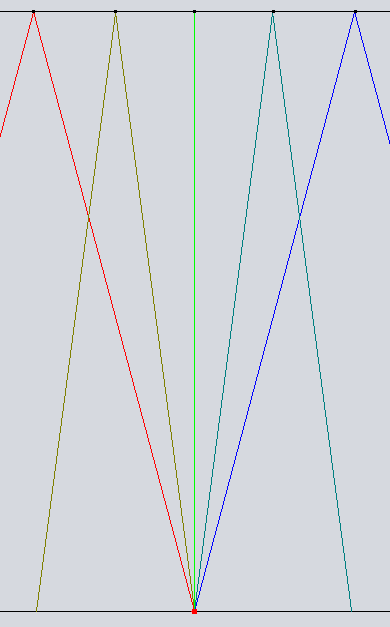
\includegraphics[scale=0.25]{pictures/Strahlenbuendel.png} 
\caption{Darstellung Wegunterschied}
\label{fig:Wegunters}
\end{wrapfigure} 
Ungeachtet des gewählten Verfahrens kommt es bei der Darstellung der Messwerte eines Scans, der auf einem Strahlenbündel basiert, immer zu dem Problem, dass Strahlen, welche einen ähnlichen Verlauf haben, sehr kleine zeitliche Differenzen zwischen ihrem Auftreffen auf dem Sender haben. 
Wie in der nebenstehenden Abbildung \ref{fig:Wegunters} zu erkennen ist, sind die zurückgelegten Strecken, und damit die benötigte Zeit der einzelnen Strahlen, besonders wenn man noch kleinere Streuwinkel wählt, gering. 
Die im Diagramm dargestellten Werte überlappen sich, doch dies entspricht nicht der Realität. 
Durch die Annahme, dass jeder Strahl einen gewissen Teil der kinetischen Energie, die in Form einer Schallwelle in den Körper abgegeben wird, repräsentiert, sollten fast gleichzeitige Treffer nicht als solche wahrgenommen werden, sondern als ein Treffer mit höherer Intensität. 
Die Notwendigkeit einer weiteren Zusammenfassung der Messwerte ist dadurch gegeben. 
Dies erfolgt in der Methode \texttt{processScan}. \par 
\begin{wrapfigure}[28]{rH}{11.5cm}
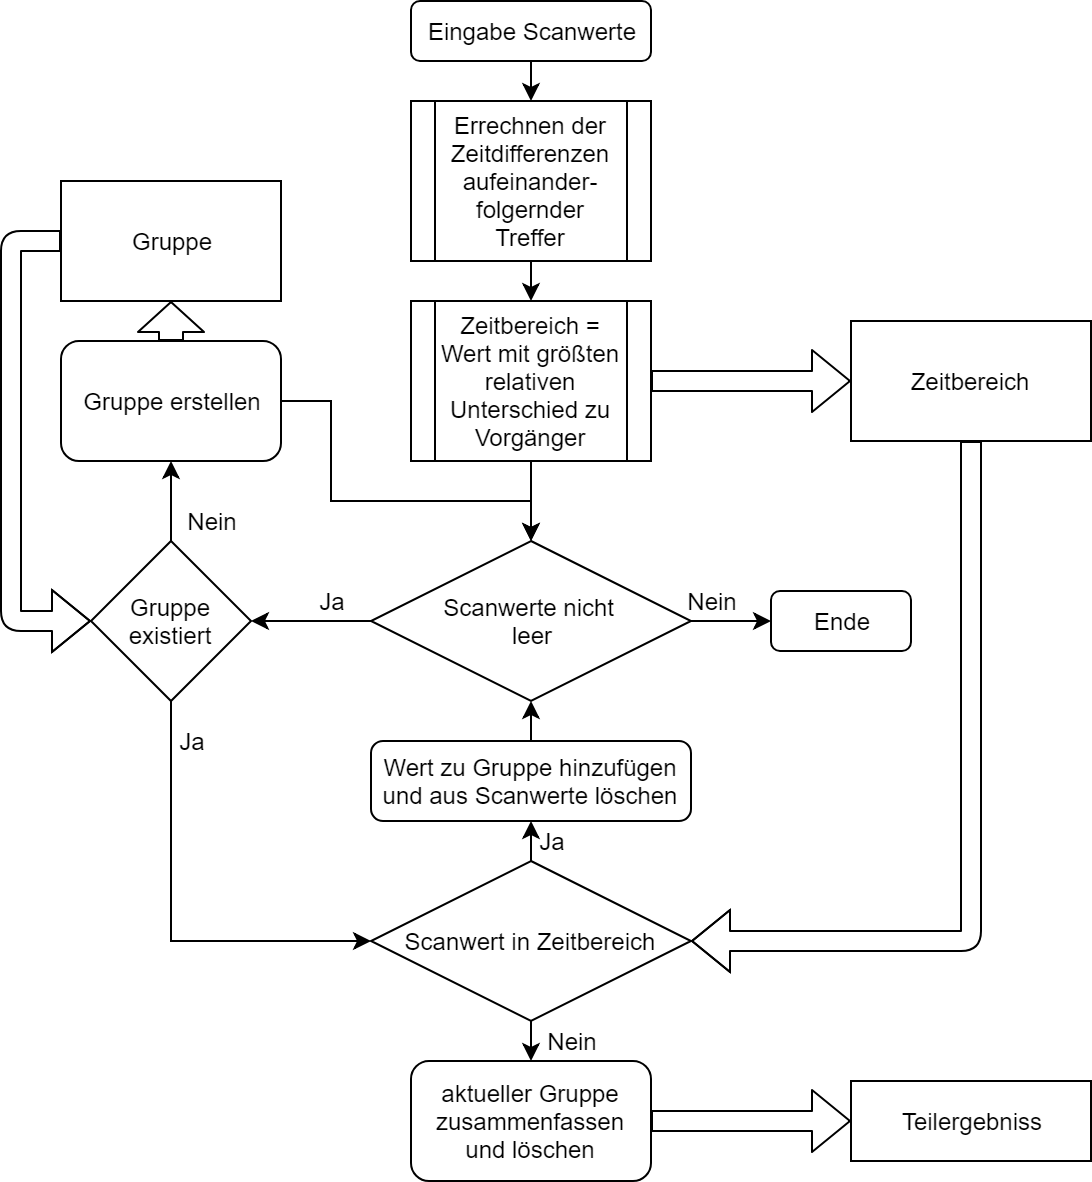
\includegraphics[scale=0.3]{pictures/Flowchart_processScan.png}
\caption{Ablauf der Funktion \texttt{processScan}}
\end{wrapfigure} 
Zuerst werden dabei alle Wertepaare aus Zeit und Intensität errechnet und in zeitlicher Abfolge sortiert. 
Zwischen zwei Wertepaaren liegt eine Zeitdifferenz, die für alle Paare errechnet und in eine Liste einsortiert wird.
Anschließend wird aus dieser Liste an Differenzen die Stelle gesucht, an der der Quotient aus zwei aufeinanderfolgenden Zeitdifferenzen am größten ist und der größere Wert der Zeitdifferenzen als sogenannter Zeitbereich definiert.
Dieser sagt aus, in welchem Abstand von einem gegebenen Treffer weitere Treffer nicht separat in das Diagramm für A-Scans eingetragen, sondern als ein Treffer zusammengefasst werden.\\
Auf Basis des Zeitbereichs werden nun alle Scanwerte in Gruppen eingeteilt. 
Ausgehend von einem Startwert werden alle folgenden Werte überprüft und solange der selben Gruppe zugeordnet, bis sie nicht mehr innerhalb des Zeitbereichs liegen. 
Die Gruppe wird dann ausgewertet, indem eine durchschnittliche Intensität der Treffer sowie eine Durch\-schnitts\-zeit errechnet wird.
Dieses Teilergebnis ist eines der neuen Wertepaare, welche dann im Diagramm für A-Scans dargestellt werden. 
Die Gruppe wird daraufhin geleert, ein neuer Wert hinzugefügt und das Verfahren wiederholt, bis alle Scanergebnisse einer Gruppe zugeordnet wurden.\\
Der genaue Ablauf der Funktion ist auch im Struktogramm unter \ref{sec:documentation} nachzulesen.

\subsection{Verwendung des Programms} %TODO für Programm neu kompilieren
\begin{figure}[h]
\centering
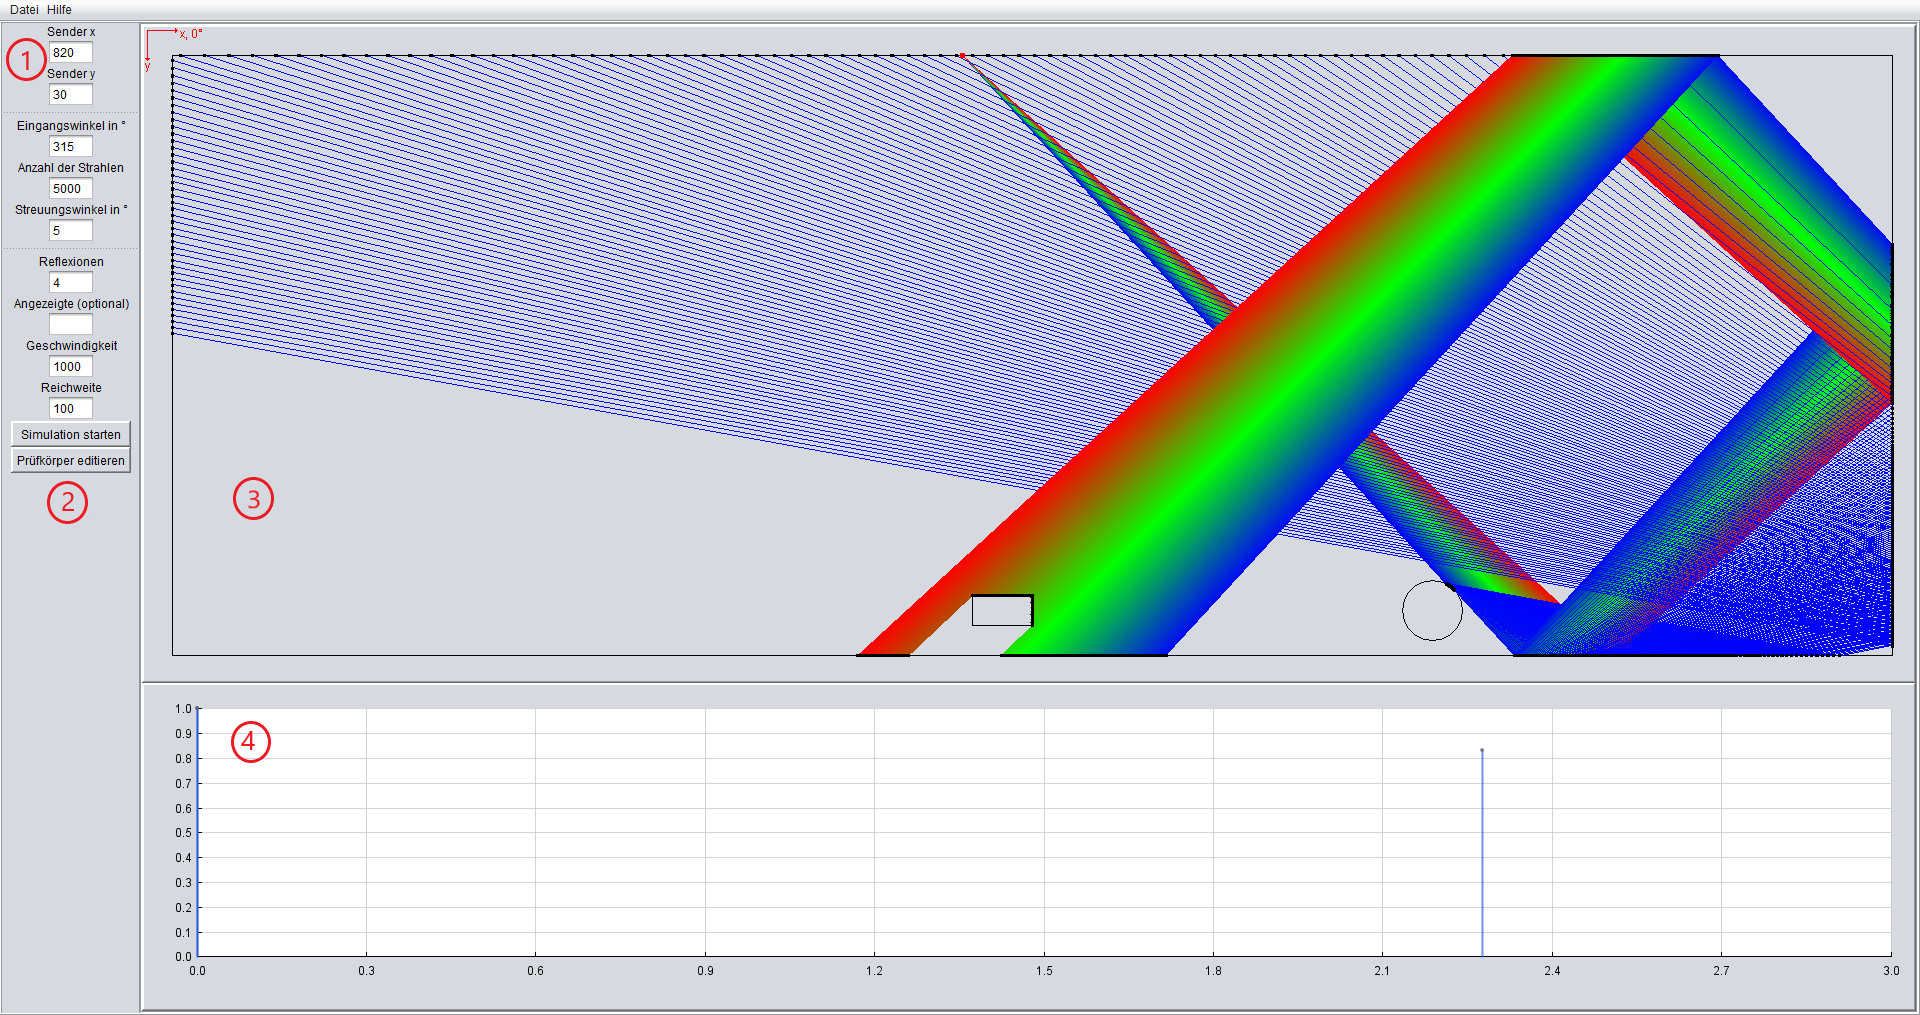
\includegraphics[scale=0.315]{pictures/MainWindow.png}
\caption{Simulationsfenster (MainWindow)}
\end{figure}
In der Sidebar für die Simulationseinstellungen (1) können Position, Ausrichtung und Art des Senders sowie weitere Parameter eingestellt werden. 
Die Position des Senders kann auch mittels der Pfeiltasten rechts und links automatisch entlang der Outline verschoben werden. 
Der Winkel des Strahls zur x-Achse kann auch mit den Plus- und Minustasten eingestellt werden. 
Mittels des Feldes \textit{Anzeige} kann man eine einzelne Reflexion anzeigen lassen. 
Der Wert dieses Feldes wird mit den Pfeiltasten nach oben und unten verstellt. 
Für all diese Kommandos muss gleichzeitig die Alt-Taste gedrückt werden.\\
Der Knopf \textit{Simulation starten} (2) führt die Simulation mit den gewählten Parametern durch. 
Dabei wird der Bearbeitungsmodus, so er aktiv ist, beendet.\\
Der Knopf \textit{Prüfkörper editieren} (2) startet den Bearbeitungsmodus. 
Dabei können kleinere Änderungen, entsprechend dem \textit{Freie Maus} Tool, am Prüfkörper vorgenommen werden,  ohne das EditorWindow zu öffnen.\\
Im Simulationspanel (3) wird die Simulation dargestellt. 
Der rote Punkt am oberen Rand des Fensters ist der Sender. 
Die schwarzen Punkte an verschiedenen Rändern von Körpern sind die Punkte, an denen Reflexionen stattfinden. 
Der Strahlenkegel wird mit einem Farbübergang deutlicher gekennzeichnet.\\
In diesem Fall wird der ursprünglich linke Teil des Strahls (die blauen Bestandteile) am Rand des Kreises zerstreut, was zu einem Echo bei der vierten Reflexion führt.\\
Das Scanpanel (4) stellt einen Graphen dar, in dem die Messergebnisse, also die Echos, dargestellt werden. 
Im obigen Beispiel ist ein Echo bei ca. 2.1 Zeiteinheiten zu sehen: die blaue Linie leicht rechts von der Markierung an der X-Achse.
\newpage
\begin{figure}[h]
\centering
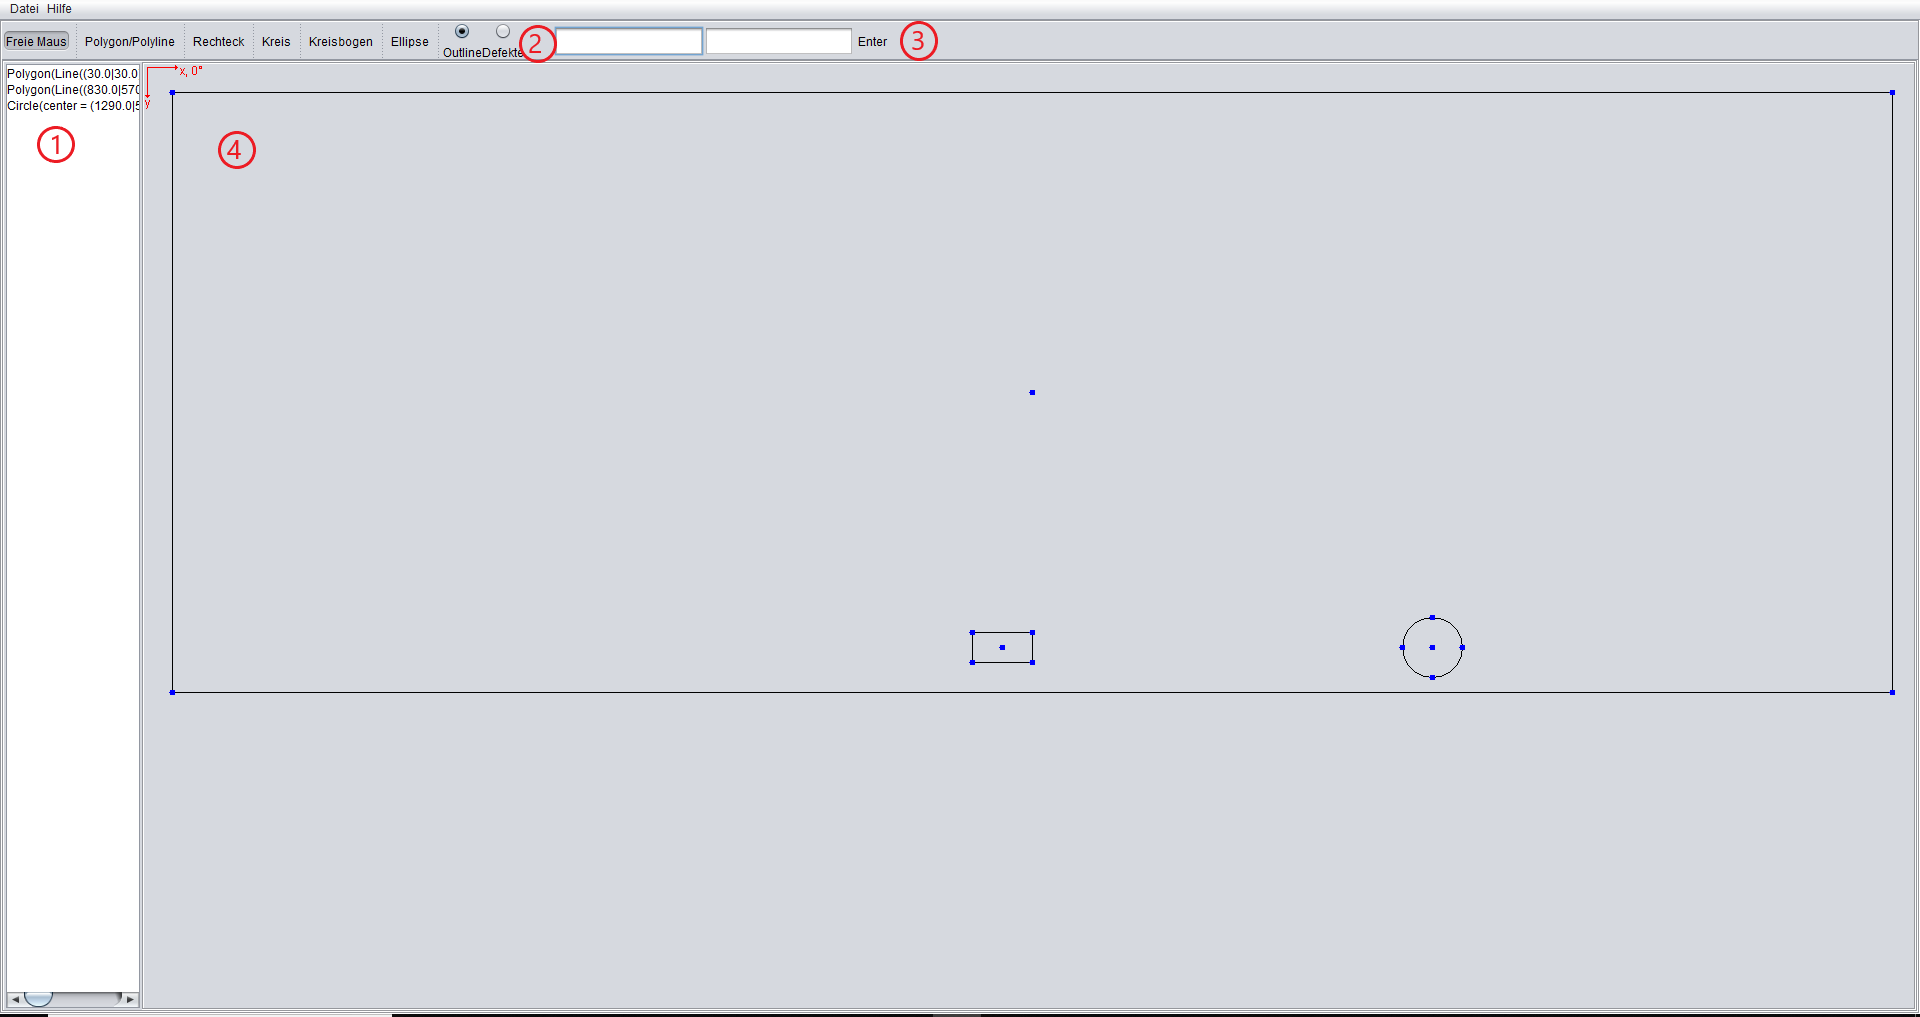
\includegraphics[scale=0.315]{pictures/EditorWindow.png}
\caption{Körpereditorfenster (EditorWindow)}
\end{figure}
Ein Sidebar (1) listet sämtliche Körper der Outline sowie Defekte auf. 
Diese Liste kann unter anderem genutzt werden, um Körper zu markieren (Linksklick), zu löschen (Entfernen) und ihre Eigenschaften zu bearbeiten (Rechtsklick oder P).\\
Letzteres beinhaltet die Möglichkeit, die geometrischen Konstruktionseigenschaften, etwa die Position der Punkte eines Polygons, und Zeicheneigenschaften, wie Linien und Flächenfarbe des Körpers, anzupassen.\\
Der Toolbar am oberen Rand (2) enthält die zur Verfügung stehenden Konstruktionstools. 
Standardmäßig ist das \textit{Freie Maus} Tool ausgewählt, welches Änderungen an existierenden Körpern ermöglicht.
Ein Klick auf einen der blauen Punkte eines Körpers markiert den Körper rot.
Sollten mehrere Punkte übereinander liegen - etwa die Ecken zweier Polygone - kann der ausgewählte Körper durch mehrfaches Klicken auf den Punkt gewechselt werden.\\
Jeder Punkt entspricht einer Eigenschaft des Körpers und das Verschieben hat entsprechende Effekte.
Ein Polygon verfügt z.B. über eine beliebige Zahl an Eckpunkten und einen Mittelpunkt, der alle Eckpunkte in die selbe Richtung um die selbe Distanz verschiebt.
Weiterhin kann man den gewählten Körper mit der linken und rechten Pfeiltaste sowie der Alt-Taste rotieren.\\
Die anderen Tools werden verwendet, indem eine Reihe von Punkten auf der Zeichenfläche (4) angeklickt wird.
Je nach Tool bestimmen diese dann die Konstruktion des Körpers.
Im Fall des \textit{Polygon} Tools entspricht jeder Klick einem Eckpunkt und ein erneuter Klick auf den ersten Punkt oder ein Klick der mittleren Maustaste beendet die Konstruktion.
In jedem Tool kann die Konstruktion außerdem mit der rechten Maustaste vorzeitig abgebrochen werden. \\
Das \textit{Rechteck} Tool hilft bei der Konstruktion der gleichnamigen regelmäßigen Vierecke, was zwar theoretisch aber oft nur schwierig mit dem \textit{Polygon} Tool möglich ist. 
Dazu wird eine Linie zwischen den ersten zwei Punkten konstruiert. 
Das Klicken der mittleren Maustaste konstruiert dann ein Rechteck mit Seiten parallel zu den Koordinatenachsen und der Linie als Diagonale. 
Fügt man jedoch einen dritten Punkt hinzu, wird ein schiefes Rechteck konstruiert.
Die Höhe des dritten Punktes über besagter Linie ist die Höhe des Rechtecks und die Linie dessen Grundseite.\\
Die \textit{Kreis} und \textit{Kreisbogen} Tools funktionieren ähnlich.
Der erste Punkt ist in beiden Fällen der Kreismittelpunkt.
Der Abstand des zweiten Punktes vom Mittelpunkt legt den Radius fest.
Konstruiert man lediglich einen Kreis, ist seine genaue Position egal.
Bei einem Kreisbogen bestimmt die Position dieses Punktes jedoch den Startwinkel des Bogens und ein dritter Punkt die Größe des Winkels.
Liegt etwa der zweite Punkt unter einem $45^{\circ}$-Winkel zum Mittelpunkt und der dritte unter einem $135^{\circ}$-Winkel, so beträgt der Startwinkel $45^{\circ}$ und der Winkelumfang $135-45=90^{\circ}$. \\
Zuletzt ermöglicht das \textit{Ellipse} Tool die Konstruktion der gleichnamigen Körper.
Die ersten beiden Punkte sind dabei die Brennpunkte der Ellipse und legen auch ihre längere Achse fest.
Der dritte Punkt bestimmt dann ihre Exzentrizität, indem eine Ellipse ermittelt wird, auf der dieser liegt.
Da die beiden Brennpunkte auf der längeren Achse liegen, ist die Exzentrizität jedoch durch den Abstand der Brennpunkte nach oben beschränkt.\\
Unabhängig vom gewählten Tool muss gewählt werden, ob die konstuierten Körper der Outline oder den Defekten hinzugefügt werden sollen. 
Dies kann über die beiden Radiobuttons rechts von den Tools festgelegt werden.
Um Ungenauigkeiten durch beliebiges Klicken auf der Zeichenfläche zu vermeiden, existiert außerdem ein Feld für die exakte Eingabe der Koordinaten eines Punktes (3).
Der nebenstehende Knopf führt dann automatisch einen Klick bei den gegebenen Koordinaten aus.

\newpage
\section{Zusammenfassung}
% Bogen zur Einleitung
    % Röntgen geht nicht -> Ultraschall
% präzise, wesentliche Darstellung der Arbeitsergebnisse
    % Information -> Verstehen, Vergleichen
    % Planung und Umsetzung des Simulationsprogramms
    % Verwendung Prüfplanung
    % Verwendung Hypothesenverifizierung
% Bezug Zielstellungen, pseudo-kritisch
    % check, check, check, check
    % aber: Programm nur 2d -> Zeitproblem
% Bezug Erweiterungsmöglichkeiten
    % 3d
    % Materialien
% Schluss: elegant, nicht schwülstig
    

Ein Brückenträger, Schienen oder ein Ölpipeline-Segment - all diese Bauteile sind häufig anzutreffen, können aber mit dem Röntgenverfahren nicht geprüft werden.
Aufgrund ihrer Größe und Unbeweglichkeit muss hierbei ein mobil durchzuführendes Verfahren eingestzt werden, welches dennoch eine Prüfung auf innere Fehler, vergleichbar mit der Durchstrahlungsmethode, ermöglicht.\\
So lassen sich die primären Vorzüge der Ultraschallprüfung zusammenfassen.
Doch, wenn das Verfahren die selbe Genauigkeit wie eine Röntgen-Untersuchung bietet, dabei jedoch kostengünstiger und weniger gefährlich ist, warum ersetzt es diese dann nicht vollständig?
Mit dieser Frage haben wir uns im Rahmen dieser Arbeit beschäftigt, um die Nachteile %TODO Probleme?
des Verfahrens zu erkennen.
Dabei haben wir vor allem das Problem der Prüfplanung identifiziert.
%Die Interpretaition der Ergebnisse ist oft schwierig - im Gegensatz zu den selbst für Laien nachvollziehbaren Röntgenaufnahmen sind die A-Scans einer Ultraschallprüfung, grade in komplexeren Szenarien, nur mit einem fundierten Fachwissen zu deuten.
Die Interpretaition der Ergebnisse ist oft schwierig, da die zeitlich versetzt auftretenden Echos erst in Zusammenhang mit den Abmessungen des Prüfkörpers und der Position und Ausrichtung des Prüfkopfes zur Identifikation von Fehlern genutzt werden können. Im Gegensatz dazu sind Röntgenaufnahmen selbst hochkomplexer Geometrien häufig für Laien auf einen Blick nachvollziehbar.\\
Um diesem Missstand entgegen zu wirken, haben wir ein Programm zur Simulation Ultraschall-basierter zerstörungsfreier Materialprüfung entwickelt.
%TODO Missstand ersetzen
Dieses erfüllt heute unsere grundlegende Zielstellung, regelmäßige zweidimensionale Geometrien und einzelne Strahlengänge zu simulieren.
Im Laufe der Arbeit erweiterten wir das Programm außerdem um komplexe Geomtrien sowie die Simulation eines Strahlenbündels.\\
Die Kombination dieser Funktionen erlaubt den Einsatz des Programms für die Prüfplanung.
Durch Verschieben des Senders und die Feineinstellung des Einstrahlungswinkels kann die richtige Ausgangssituation für vielfältige Prüfungsszenarien gefunden werden. \\
Ein weiteres erreichtes Ziel ist die Verwendung zur Hypothesenverifizierung.
Anders als bei der Prüfplanung sollen hier die aus einer bereits durchgeführten Prüfung abgeleiteten Vermutungen über Position, Form und Größe von Fehlern bestätigt oder entkräftet werden.
Dazu wird die erwartete Situation im Programm nachgestellt und simuliert. 
Mithilfe der Funktion, basierend auf einem ermittelten Strahlenverlauf, die Peaks eines A-Scans anzuzeigen, kann der Nutzer durch Abgleich mit den realen Messergebnisse auf den Wahrheitsgehalt seiner Hypothese schließen.\\
Obwohl wir die Arbeit somit als erfolgreich bezeichnen können, konnten wir nicht alle Erweiterungsmöglichkeiten, die wir uns zu Beginn überlegten, umsetzen.
Diese stellen zugleich die vielversprechendsten Ansätze für eine Fortführung des Projekts dar.
Zum einen wäre eine Erweiterung der Algorithmen um regelmäßige dreidimensionale Geometrien denkbar, wenn auch sehr zeitaufwendig.
Zum anderen lässt sich der Realismus der vorhandenen, zweidimensionalen Simulationen erhöhen, indem man Materialübergänge und materialspezifische Schallgeschwindigkeiten einführt, wodurch ein weites Feld an zusätzlichen Anwendungsmögichkeiten erschlossen wird.\\
[kreativer Schluss, Bezug zu Zulunft des Verfahrens?]
\newpage
\section{Anhang}

\subsection{Vollständige Herleitung aller verwendeten Berechnungsformeln} \label{sec:AnhangHerlFormel}
Grundbestandteil unseres Programms ist es, Strahlen mit regelmäßigen zweidimensionalen Körpern zu schneiden. 
Viele Verfahren sind dafür bereits bekannt, für die Anwendung innerhalb eines Simulationsprogramms sind diese allerdings eher selten geeignet.\\
Für die Berechnung gibt es im Allgemeinen gegebene Größen, aus denen sich die Ergebnisse ableiten lassen. Doch im Gegensatz zum Menschen sind Computer nicht in der Lage, einfache Fälle selbst zu erkennen, sondern benötigen im Idealfall eine Berechnungsformel zur Bestimmung eines Wertes, um laufzeiteffizient arbeiten zu können.

\subsubsection*{Herleitung der Formel für Geraden}

\begin{figure}[h]
\centering
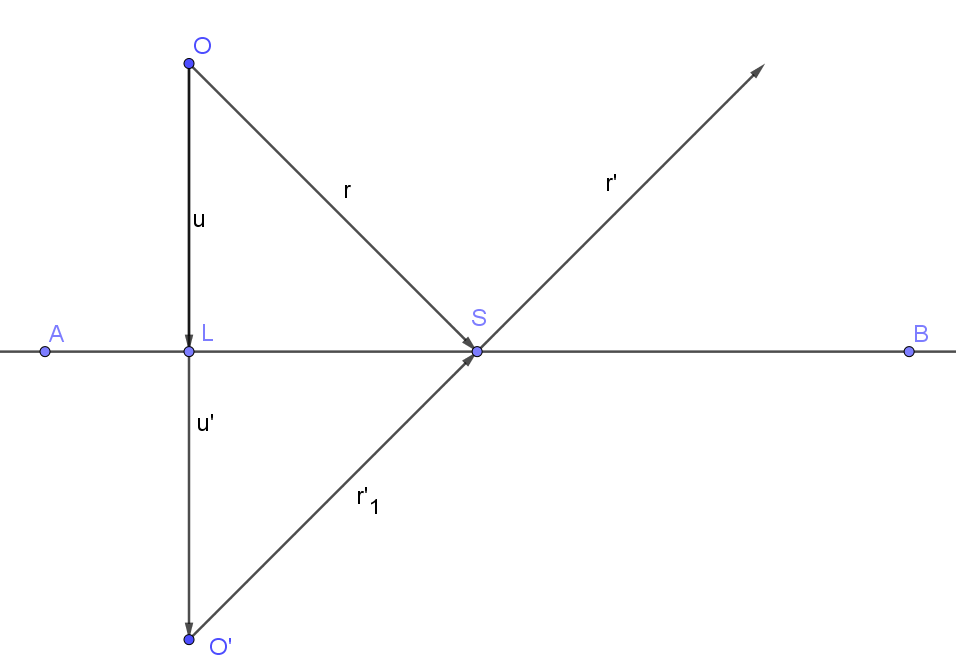
\includegraphics[scale=0.5]{pictures/LineRef.png}
\caption{Reflexion an einer Geraden}
\end{figure}

gegeben:
\begin{subequations} 
\begin{align}
g:~ \vec{x} &= \vec{a} + f \cdot \vec{AB} := \vec{a} + f \cdot \vec{v} \wedge f \in \mathds{R} \label{eq:Gg1} \\ 
s:~ \vec{x} &= \vec{o} + h \cdot \vec{r} \wedge h \in \mathds{R} \label{eq:Gg2}
\end{align}
\end{subequations}

gesucht:
\begin{subequations}
\begin{align}
S(Sx|Sy)~~~~~~~~~ \nonumber \\
s':~ \vec{x} = \vec{s} + i \cdot \vec{r'} \wedge i \in \mathds{R} \nonumber
\end{align}
\end{subequations}

\newpage
Lösung:
\begin{center}
\ref{eq:Gg1} gleichsetzen mit \ref{eq:Gg2}
\end{center}
\begin{equation*}
\begin{split} 
\vec{a} + f \cdot \vec{v} &= \vec{o} + h \cdot \vec{r}
\end{split}
\end{equation*}
\begin{equation*}
\begin{split}
h_1 &= \frac{a_x + f \cdot v_x - o_x}{r_x} \\
h_2 &= \frac{a_y + f \cdot v_y - o_y}{r_y} \\
\end{split}
\end{equation*}
\begin{equation*}
\begin{split}
h_1 &= h_2 \\
\frac{a_x + f \cdot v_x - o_x}{r_x} &= \frac{a_y + f \cdot v_y - o_y}{r_y} \\
f \cdot \frac{v_x}{r_x} - f \cdot \frac{v_y}{r_y} &= \frac{a_y - o_y}{r_y} - \frac{a_x - o_x}{r_x} \\
f(\frac{v_x \cdot r_y - v_y \cdot r_x}{r_x \cdot r_y}) &= \frac{a_y \cdot r_x - o_y \cdot r_x - a_x \cdot r_y + o_x \cdot r_y}{r_x \cdot r_y} 
\end{split}
\end{equation*}

\begin{equation*}
\begin{split}
f &= \frac{a_y \cdot r_x - o_y \cdot r_x - a_x \cdot r_y + o_x \cdot r_y}{v_x \cdot r_y - v_y \cdot r_x} \\
\vec{s} &= \vec{a} + f \cdot \vec{v}
\end{split}
\end{equation*}
Um nun an der Geraden reflektieren zu können, müssen der Lotfußpunkt $L$ von $O$ auf $g$  und der Spiegelpunkt $O'$ bestimmt werden.
\begin{equation*}
\begin{split}
\vec{n}~ &\bot ~\vec{v} \\
\vec{n} &= \begin{pmatrix} -v_y \\ v_x \end{pmatrix} \\
\end{split}
\end{equation*}
Durch das Schneiden der beiden Geraden $g$ (\ref{eq:Gg1}) und $n: \vec{x} = \vec{o} + f' \cdot \vec{n} \wedge f' \in \mathds{R}$ ergibt sich der Faktor $f'$, woraus $L$ und $O'$ folgen.
\begin{equation*}
\begin{split}
g &= n \\
\vec{l} &= \vec{o} + f' \cdot \vec{n} \\
\vec{u} &= \vec{l} - \vec{o} \\
\vec{o'} &= \vec{o} + 2 \cdot \vec{u} \\
\vec{r'} &= \vec{o'} - \vec{s} \\
\end{split}
\end{equation*}
Somit erhalten wir das Ergebnis $s'$ mit:
\begin{equation*}
\underline{\underline{s':~ \vec{x} = \vec{s} + i \cdot \vec{r'} \wedge i \in \mathds{R}}}
\end{equation*}

\newpage
\subsubsection*{Herleitung der Formel für Kreise}

\begin{figure}[h]
\centering
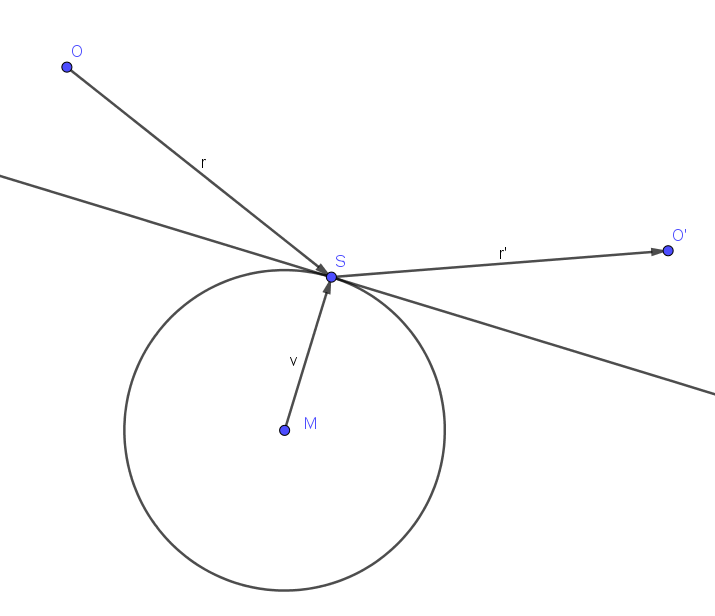
\includegraphics[scale=0.5]{pictures/CircleRef.png}
\caption{Reflexion an einem Kreis}
\end{figure}

gegeben:
\begin{subequations}
\begin{align}
K:~ \vec{x} &= \vec{m} + \vec{c} \label{eq:Kg1}\\
|\vec{v}| &= r \label{eq:Kg2} \\
s:~ \vec{x} &= \vec{o} + \lambda \cdot \vec{r} \nonumber
\end{align}
\end{subequations}

gesucht:
\begin{subequations}
\begin{align}
S(&S_x|S_y) \nonumber \\
s':~ \vec{x} &= \vec{s} + \lambda \cdot \vec{r'} \nonumber 
\end{align}
\end{subequations}

Lösung:
\begin{equation*}
\begin{split}
\ref{eq:Kg1}: &\\
s_x &= m_x + v_x \\
 &= o_x + \lambda \cdot r_x \\
v_x &= s_x - m_x \\
s_y &= m_y + v_y \\
 &= o_y + \lambda \cdot r_y \\
v_y &= s_y - m_y \\
\ref{eq:Kg2}: & \\
r &= \sqrt{{v_x}^2 + {v_y}^2} \\
r^2 &= {v_x}^2 + {v_y}^2 \\
 &= {(s_x - m_x)}^2 + {(m_y - s_y)}^2 
\end{split}
\end{equation*}

\begin{equation*}
\begin{split}
r^2 &= {(o_x + \lambda \cdot r_x - m_x)}^2 + {(o_y + \lambda \cdot r_y - m_y)}^2 \\
 &= {o_x}^2 + 2\lambda\cdot r_x \cdot o_x - 2 \cdot o_x \cdot m_x + \lambda^2 \cdot {r_x}^2 - 2\lambda \cdot m_x \cdot r_x + {m_x}^2 \\
 & ~~~+{o_y}^2 + 2\lambda\cdot r_y \cdot o_y - 2 \cdot o_y \cdot m_y + \lambda^2 \cdot {r_y}^2 - 2\lambda \cdot m_y \cdot r_y + {m_y}^2 \\
0 &= \lambda^2 \cdot ({r_x}^2 + {r_y}^2) + \lambda \cdot (2 \cdot r_x \cdot o_x - 2 \cdot r_x \cdot m_x + 2 \cdot r_y \cdot m_y - 2 \cdot r_y \cdot m_y) \\
 & ~~~+({o_x}^2 - 2 \cdot o_x \cdot m_x + {m_x}^2 + {o_y}^2 - 2 \cdot o_y \cdot m_y + {m_y}^2 - r^2) \\
 &= \lambda^2 \cdot ({r_x}^2 + {r_y}^2) + \lambda \cdot (2 \cdot r_x \cdot (o_x - m_x) + 2 \cdot r_y \cdot (o_y - m_y)) + ({(o_x - m_x)}^2 + {(o_y - m_y)}^2 - r^2) \\
 &= \lambda^2 + \lambda \cdot \dfrac{2 \cdot r_x \cdot (o_x - m_x) + 2 \cdot r_y \cdot (o_y - m_y)}{{r_x}^2 + {r_y}^2} + \dfrac{{(o_x - m_x)}^2 + {(o_y - m_y)}^2 - r^2}{{r_x}^2 + {r_y}^2}
\end{split}
\end{equation*}

Mit der Lösungsformel für binomische Gleichungen 
\begin{equation*}
x_{1/2} = \dfrac{-p}{2} \pm \sqrt{{(\dfrac{p}{2})}^2 - q}
\end{equation*}
ergibt sich als Lösung für $\lambda_{1/2}$ mit
\begin{equation*}
\begin{split}
p_{bin} &= \dfrac{2 \cdot r_x \cdot (o_x - m_x) + 2 \cdot r_y \cdot (o_y - m_y)}{{r_x}^2 + {r_y}^2} \\
q_{bin} &= \dfrac{{(o_x - m_x)}^2 + {(o_y - m_y)}^2 - r^2}{{r_x}^2 + {r_y}^2}
\end{split}
\end{equation*}
falls ${(\dfrac{p_{bin}}{2})}^2 - q_{bin} \geq 0$ gilt:
\begin{equation*}
\begin{split}
\lambda_1 &= \dfrac{-p_{bin}}{2} + \sqrt{{(\dfrac{p_{bin}}{2})}^2 - q_{bin}} \\
\lambda_2 &= \dfrac{-p_{bin}}{2} - \sqrt{{(\dfrac{p_{bin}}{2})}^2 - q_{bin}}
\end{split}
\end{equation*}
Daraus ergeben sich zwei Schnittpunkt $S_{1/2}$ mit $\vec{s_{1/2}} = \vec{o} + \lambda_{1/2} \cdot \vec{r}$, für die der Schnittpunkt mit dem kleineren Abstand $d(S_{1/2}, O) = \sqrt{{(S_{1/2, x} - Ox)}^2 + {(S_{1/2, y} - Oy)}^2}$ ausgewählt wird, um daran eine Tangente anzulegen, an welcher nach der Formel für Geradenreflexion der Strahl $s$ zu $s'$ reflektiert wird. Falls die Ungleichung nicht stimmt, schneidet der Strahl die Gerade nicht.




\newpage
\subsubsection*{Herleitung der Formel für Ovale}

\begin{figure}[h]
\centering
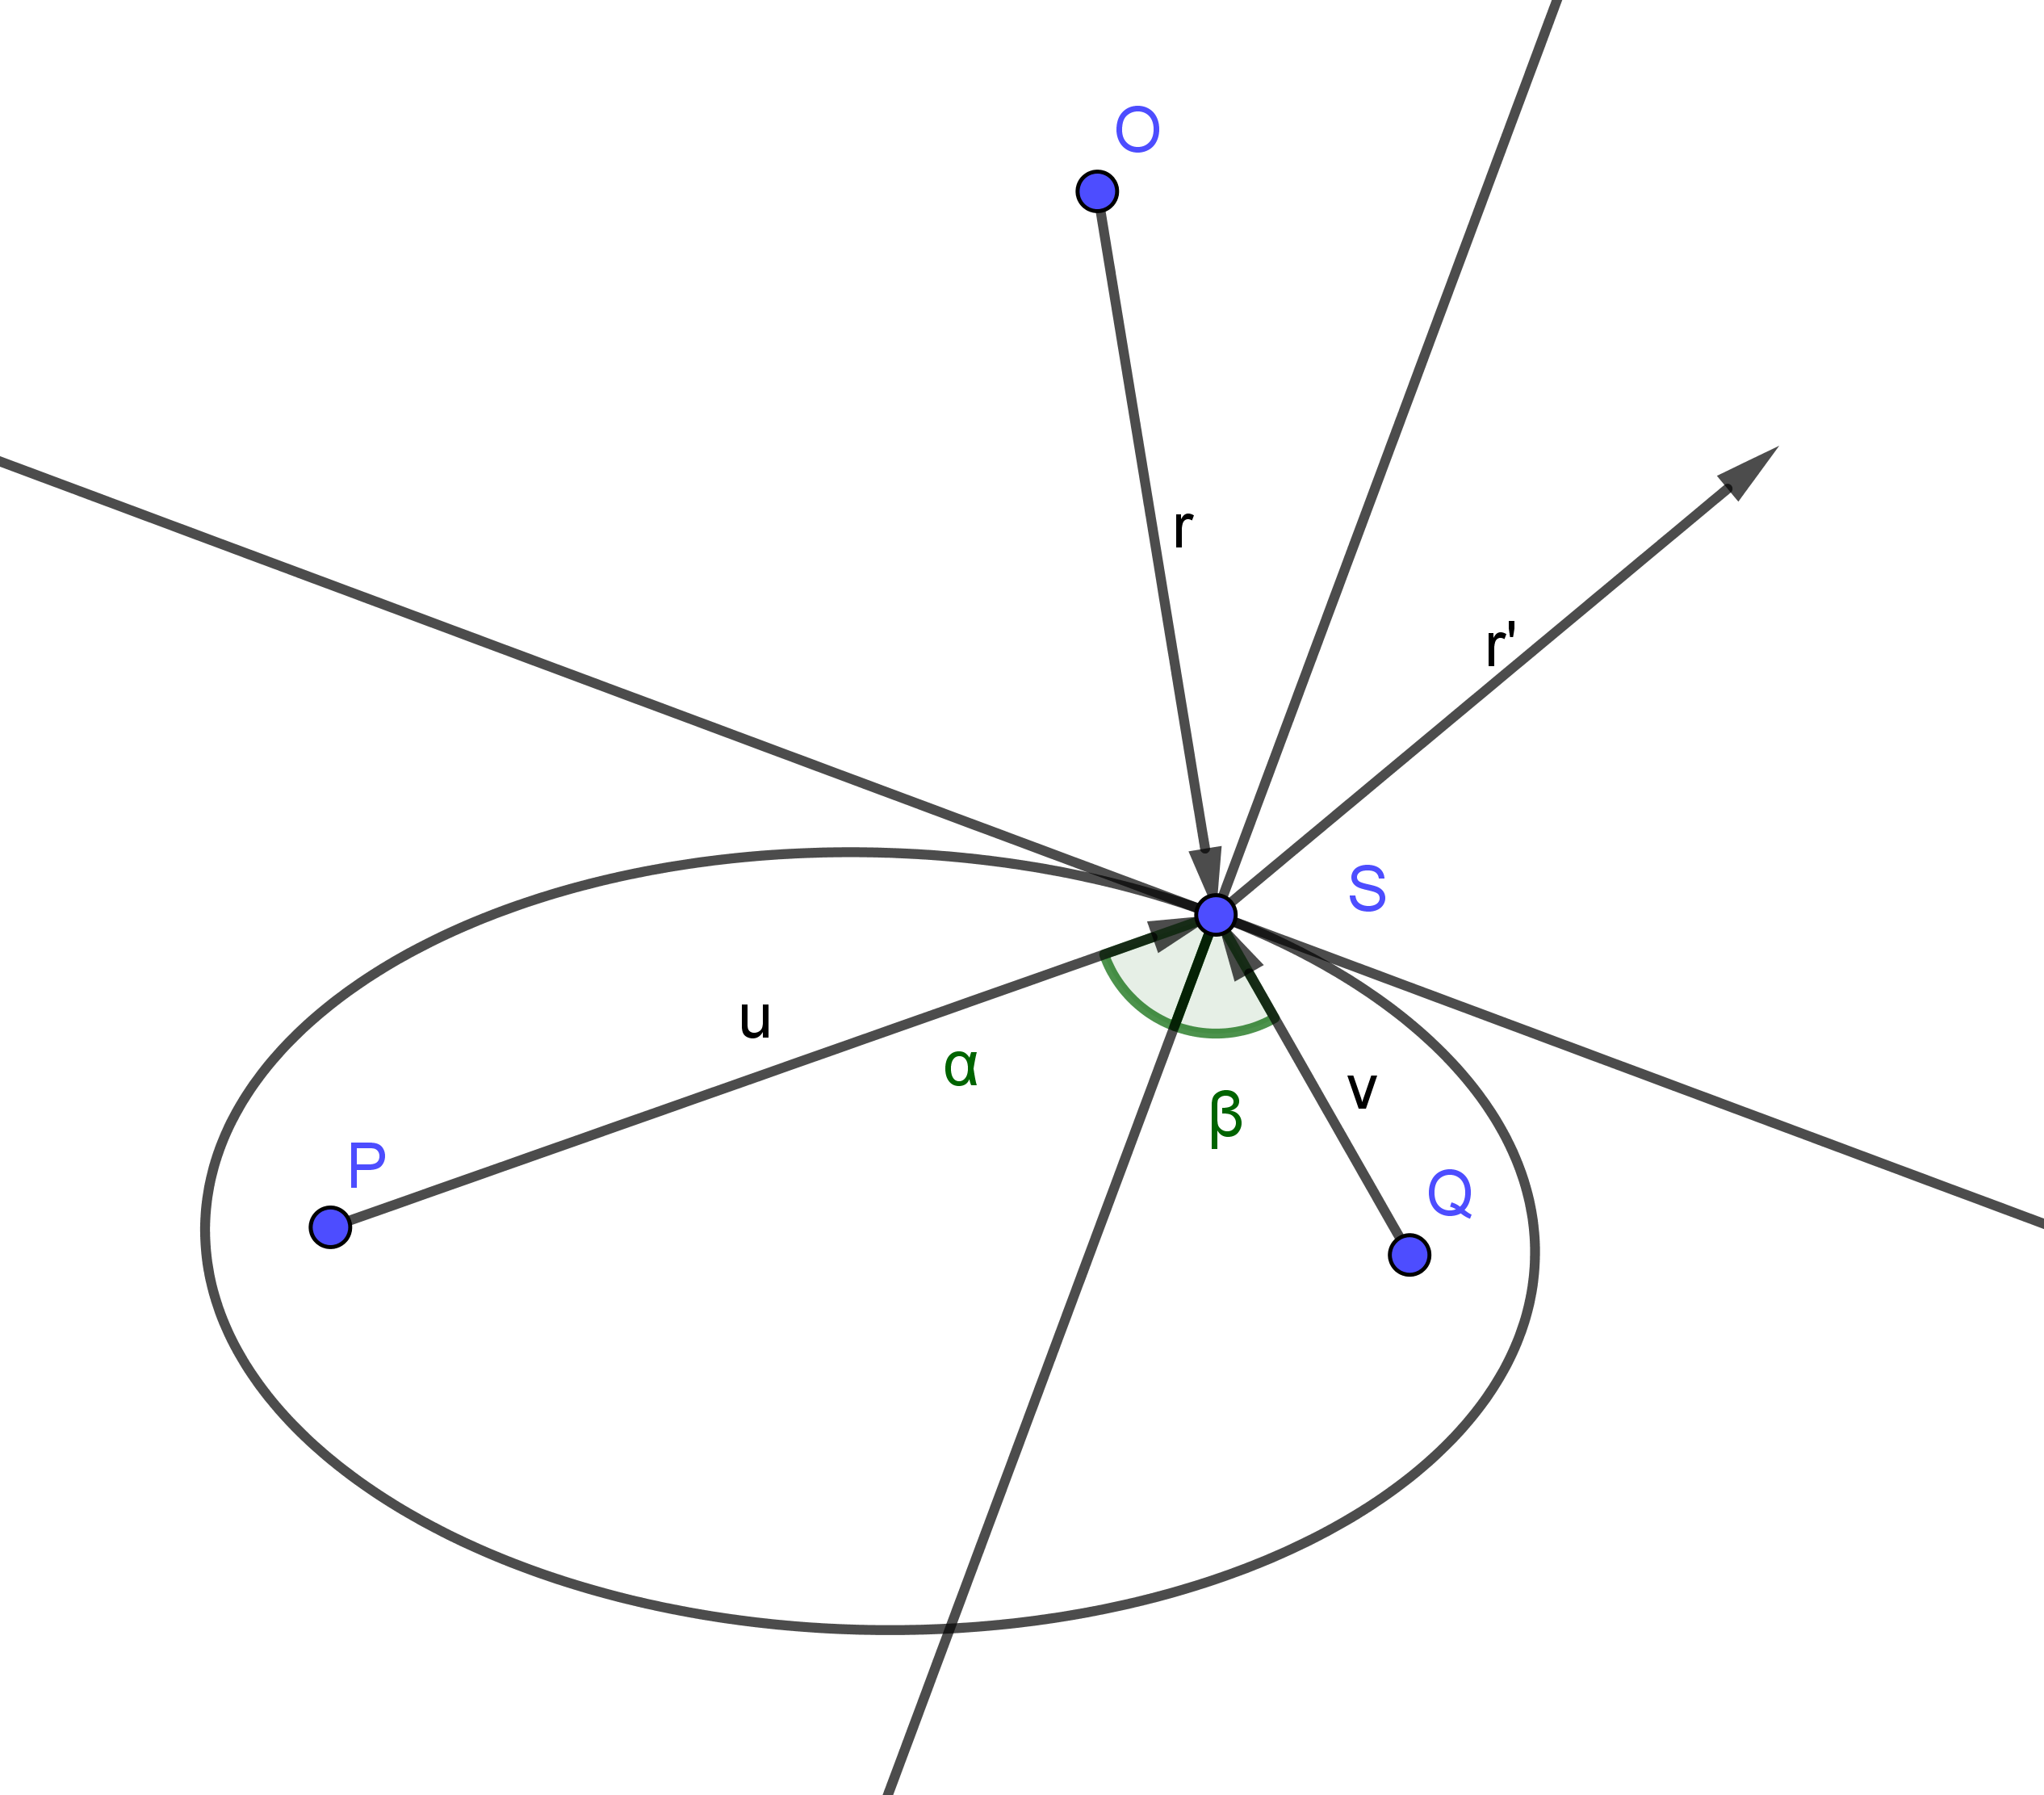
\includegraphics[scale=1]{pictures/OvalRef.png}
\caption{Reflexion an einem Oval}
\end{figure}

gegeben:
\begin{subequations}
\begin{align}
s:~ \vec{x} &= \vec{o} + \lambda \cdot \vec{r} \wedge f \in \mathds{R} \nonumber \\
E:~ \vec{x} &= \vec{p} + \vec{u} = \vec{q} + \vec{v} \nonumber  \\
e &= |\vec{u}| + |\vec{v}| \nonumber
\end{align}
\end{subequations}

gesucht:
\begin{subequations}
\begin{align}
S(Sx|Sy)~~~~~~~~~~ \nonumber  \\
t:~ \vec{x} = \vec{s} + h \cdot \vec{t} \wedge h \in \mathds{R} \nonumber 
\end{align}
\end{subequations}

Lösung: \\
Um das Oval mit dem Strahl zu schneiden, müssen diese beiden gleichgesetzt werden. Es ergibt sich folgendes Gleichungssystem:
\begin{equation*}
\begin{split}
\vec{o} + \lambda \cdot \vec{r} &= \vec{p} + \vec{u} \\
\vec{o} + \lambda \cdot \vec{r} &= \vec{q} + \vec{v} \\
\vec{p} + \vec{u} &= \vec{q} + \vec{v} \\
|\vec{u}| + |\vec{v}| &= e
\end{split}
\end{equation*}
Für dieses findet man zwei Lösungen, die sich wie bei den anderen Geometrien auch durch Umformen und schrittweises ineinander-Einsetzen der Ausgangsgleichungen ergeben. Jedoch verzichten wir aufgrund der Größe der Formel darauf, jeden Teilschritt mitzuführen, und beschränken uns lediglich auf das Ergebnis.



\begin{equation*}
\lambda_1 = \dfrac{- M_1}{2 \cdot (e^{2} \cdot (r_x^{2} + r_y^{2}) - (P_x \cdot r_x + P_y \cdot r_y - Q_x \cdot r_x - Q_y \cdot r_y)^{2})}
\end{equation*}
\begin{equation*}
\begin{aligned}
M_1 &= e \cdot [e^{4} \cdot (r_x^{2} + r_y^{2}) - 2 \cdot e^{2} \cdot (2 \cdot O_x^{2} \cdot r_y^{2} - 2 \cdot O_x \cdot (2 \cdot O_y \cdot r_x + P_x \cdot r_y - P_y \cdot r_x + Q_x \cdot r_y - Q_y \cdot r_x) \\
& \cdot r_y + 2 \cdot O_y^{2} \cdot r_x^{2} + 2 \cdot O_y \cdot (P_x \cdot r_y - P_y \cdot r_x + Q_x \cdot r_y - Q_y \cdot r_x) \cdot r_x + P_x^{2} \cdot (r_x^{2} + r_y^{2}) \\
&- 2 \cdot P_x \cdot (Q_x \cdot r_x + Q_y \cdot r_y) \cdot r_x + P_y^{2} \cdot (r_x^{2} + r_y^{2}) - 2 \cdot P_y \cdot (Q_x \cdot r_x + Q_y \cdot r_y) \cdot r_y \\
&+ (Q_x^{2} + Q_y^{2}) \cdot (r_x^{2} + r_y^{2})) + (4 \cdot O_x^{2} \cdot r_y^{2} - 4 \cdot O_x \cdot (2 \cdot O_y \cdot r_x + P_x \cdot r_y - P_y \cdot r_x + Q_x \cdot r_y - Q_y \cdot r_x) \\
&\cdot r_y + 4 \cdot O_y^{2} \cdot r_x^{2} + 4 \cdot O_y \cdot (P_x \cdot r_y - P_y \cdot r_x + Q_x \cdot r_y - Q_y \cdot r_x) \cdot r_x + P_x^{2} \cdot (r_x^{2} + r_y^{2}) \\
&- 2 \cdot P_x \cdot (Q_x \cdot (r_x^{2} - r_y^{2}) + 2 \cdot Q_y \cdot r_x \cdot r_y) + P_y^{2} \cdot (r_x^{2} + r_y^{2}) - 2 \cdot P_y \cdot (2 \cdot Q_x \cdot r_x \cdot r_y \\
&- Q_y \cdot (r_x^{2} - r_y^{2})) + (Q_x^{2} + Q_y^{2}) \cdot (r_x^{2} + r_y^{2})) \cdot (P_x^{2} - 2 \cdot P_x \cdot Q_x + P_y^{2} - 2 \cdot P_y \cdot Q_y + Q_x^{2} + Q_y^{2})]^{\frac{1}{2}} \\
&+ e^{2} \cdot (2 \cdot O_x \cdot r_x + 2 \cdot O_y \cdot r_y - P_x \cdot r_x - P_y \cdot r_y - Q_x \cdot r_x - Q_y \cdot r_y) - (2 \cdot O_x \cdot (P_x - Q_x) \\
&+ 2 \cdot O_y \cdot (P_y - Q_y) - P_x^{2} - P_y^{2} + Q_x^{2} + Q_y^{2}) \cdot (P_x \cdot r_x + P_y \cdot r_y - Q_x \cdot r_x - Q_y \cdot r_y)
\end{aligned}
\end{equation*}

\begin{equation*}
\lambda_2 = \dfrac{M_2}{2 \cdot (e^{2} \cdot (r_x^{2}+r_y^{2})-(P_x \cdot r_x+P_y \cdot r_y-Q_x \cdot r_x-Q_y \cdot r_y)^{2})}
\end{equation*}
\begin{equation*}
\begin{aligned}
M_2 &= e \cdot [e^{4} \cdot (r_x^{2} + r_y^{2}) - 2 \cdot e^{2} \cdot (2 \cdot O_x^{2} \cdot r_y^{2} - 2 \cdot O_x \cdot (2 \cdot O_y \cdot r_x + P_x \cdot r_y - P_y \cdot r_x + Q_x \cdot r_y - Q_y \cdot r_x) \\
& \cdot r_y + 2 \cdot O_y^{2} \cdot r_x^{2} + 2 \cdot O_y \cdot (P_x \cdot r_y - P_y \cdot r_x + Q_x \cdot r_y - Q_y \cdot r_x) \cdot r_x + P_x^{2} \cdot (r_x^{2} + r_y^{2}) \\
& - 2 \cdot P_x \cdot (Q_x \cdot r_x + Q_y \cdot r_y) \cdot r_x + P_y^{2} \cdot (r_x^{2} + r_y^{2}) - 2 \cdot P_y \cdot (Q_x \cdot r_x + Q_y \cdot r_y) \cdot r_y \\
&+ (Q_x^{2} + Q_y^{2}) \cdot (r_x^{2} + r_y^{2})) + (4 \cdot O_x^{2} \cdot r_y^{2} - 4 \cdot O_x \cdot (2 \cdot O_y \cdot r_x + P_x \cdot r_y - P_y \cdot r_x + Q_x \cdot r_y - Q_y \cdot r_x) \\
&\cdot r_y + 4 \cdot O_y^{2} \cdot r_x^{2} + 4 \cdot O_y \cdot (P_x \cdot r_y - P_y \cdot r_x + Q_x \cdot r_y - Q_y \cdot r_x) \cdot r_x + P_x^{2} \cdot (r_x^{2} + r_y^{2}) \\
&- 2 \cdot P_x \cdot (Q_x \cdot (r_x^{2} - r_y^{2}) + 2 \cdot Q_y \cdot r_x \cdot r_y) + P_y^{2} \cdot (r_x^{2} + r_y^{2}) - 2 \cdot P_y \cdot (2 \cdot Q_x \cdot r_x \cdot r_y \\
&- Q_y \cdot (r_x^{2} - r_y^{2})) + (Q_x^{2} + Q_y^{2}) \cdot (r_x^{2} + r_y^{2})) \cdot (P_x^{2} - 2 \cdot P_x \cdot Q_x + P_y^{2} - 2 \cdot P_y \cdot Q_y + Q_x^{2} + Q_y^{2})]^{\frac{1}{2}} \\
&- e^{2} \cdot (2 \cdot O_x \cdot r_x + 2 \cdot O_y \cdot r_y - P_x \cdot r_x - P_y \cdot r_y - Q_x \cdot r_x - Q_y \cdot r_y) + (2 \cdot O_x \cdot (P_x - Q_x) \\
&+ 2 \cdot O_y \cdot (P_y - Q_y) - P_x^{2} - P_y^{2} + Q_x^{2} + Q_y^{2}) \cdot (P_x \cdot r_x + P_y \cdot r_y - Q_x \cdot r_x - Q_y \cdot r_y)
\end{aligned}
\end{equation*}

Für die Wurzel in den beiden Gleichungen gilt, dass ihr Radikant einen negativen Wert hat, wenn der Strahl das Oval nicht schneidet. Daher muss dieser Wert zuerst ausgerechnet und überprüft werden.\\
Ist der Radikant hingegen positiv, ergibt sich daraus mit $\vec{s} = \vec{o} + \lambda \cdot \vec{r}$ der Schnittpunkt $S$. Nun muss lediglich nach dem im Kapitel \ref{sec:weitereGeometrien} beschriebenen Verfahren eine Tangente durch $S$ an das Oval angelegt und daran die Reflexion durchgeführt werden.

\subsubsection*{Funktion zur Berechnung gerichteter Winkel}
%TODO vervollständigen

\subsection{Programmdokumentation}
\label{sec:documentation}
%TODO vervollständigen

\newpage
\nocite{*}
\section{Literatur- und Quellenverzeichnis}
\printbibliography[type=online, title=Internetquellen]
\printbibliography[type=book, title=Buchquellen]
\printbibliography[type=misc, title=Bildquellen]
Sämtliche anderen Bilder sind entweder Aufnahmen der Programmoberfläche oder eigens erstellte geometrische Konstruktionen und UML-Diagramme.
%TODO Tipps von Florian überprüfen
%TODO FINAL: Wortrennung an Zeilenende und Satztrennung an Seitenende prüfen -> notfalls manuell ändern

\eidesstattlicheerklaerung

\end{document}